This chapter describes hardware aspects of the Large Hadron Collider(LHC) 
and the Compact Muon Solenoid(CMS) detector. The content is heavily based on 
the chapter 1 of CMS Technical Design Report(TDR) volume 1~\cite{cmstdr1}.


\section{Large Hadron Collider} 

%Overview of accelerator, try to answer these questions;   
%\begin{itemize}
%  \item How beams are focused 
%  \item beam crossing angle 
%  \item Determination of luminosity and its uncertainty 
%\end{itemize}

In order to answer to the key question in the particle physics, 
the origin of mass, physicists constructed a high-energy 
proton-proton(hadrons) collider at CERN. The circumference of the accelator 
is about 27~km, which is large. Thus, the collider is called 
``Large Hadron collider(LHC)". 

The protons are accelerated to the desired collision energy 
going through multiple steps. 
Fig.~\ref{fig:cerncomplex} shows a schematic of the LHC complex. 
The protons are made by applying electric field to hydrogen gas
(Hydrogen atom is composed of one proton and one electron) 
in a metal cylinder. Then, the protons and electrons that constituted 
hydrogen atoms are separated. The separated protons leave 
the metal cylinder at the energy 90~\keV to be 
sent to Radio Frequency Quadrupole(QRF). QRF not only accelerates 
the protons to 750~\keV, but also provides a transverse focusing 
of the beam. The next destination is a linear accelarator(LINAC2) 
where the protons gain energy up to 50~\MeV($v=0.3c$).
The protons are then Proton Synchrotron Booster (PSB) which has 
157~m circumference. The PSB accelerates the protons to 1.4~\GeV\
before sending them to Proton Synchrotron (PS) of 628~m circumference.
PS is responsible for making 81 proton bunches with 25~ns spacing and energy of 25~\GeV($v=0.87c$),  
and send them to Super Proton Synchrotron (SPS) of which circumference is 7~km. 
SPS accelerates the proton bunches to 450~\GeV\ and finally inject them 
to LHC, and they are accelerated to the desired collision energy($v=0.999999c$). 
The lifetime of beams in LHC is around 10 hours and after that 
the protons are dumped to prepare for the next proton fill. 

%
\begin{figure}[ht!] 
\centering 
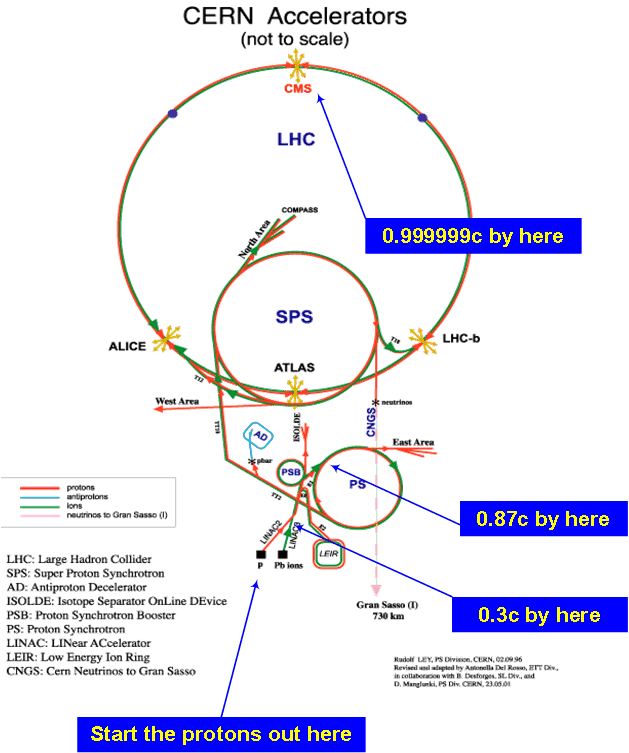
\includegraphics[width=0.99\textwidth]{figures/Cern-complex.png}
\caption{Schematic of the CERN accelerator complex.} 
\label{fig:cerncomplex} 
\end{figure} 

%Though LHC is a circular accelerator, it is not a perfect circle, 
%but consists of eight 2.45 km arcs and eight 545 m straight insersions. 
%Each arc contains 154 dipole magnets where protons are bent. 

To reach very high collision energy with a fixed size of accelerator, 
the magnetic field that bends the protons should be very high. 
In order to operate at the design proton energy of LHC (7~\TeV), 
the magnetic field should be 8.33~T. This magnetic field is too high, 
LHC uses dipole magnets using electromagnets. For an electronmagnet 
to have a high magnetic field, the current that runs in the rounding coil 
should be high. But, practically this is not easy because the coils will burn 
at high current due to its resistence. LHC dipole magnets use 
niobium-titanium(NbTi) cables with a current 11850~A at the temperature 1.9~K.
The extremely low temperature, 1.9~K, at which the coil becomes a superconductor
is achieved using superfluid helium.  
Fig.~\ref{fig:SCdipole} shows the inner structure, cross section and magnetic field map of
an LHC cryodipole.

%The bunch size of the LHC proton beam 

%
\begin{figure}[ht!] 
\centering 
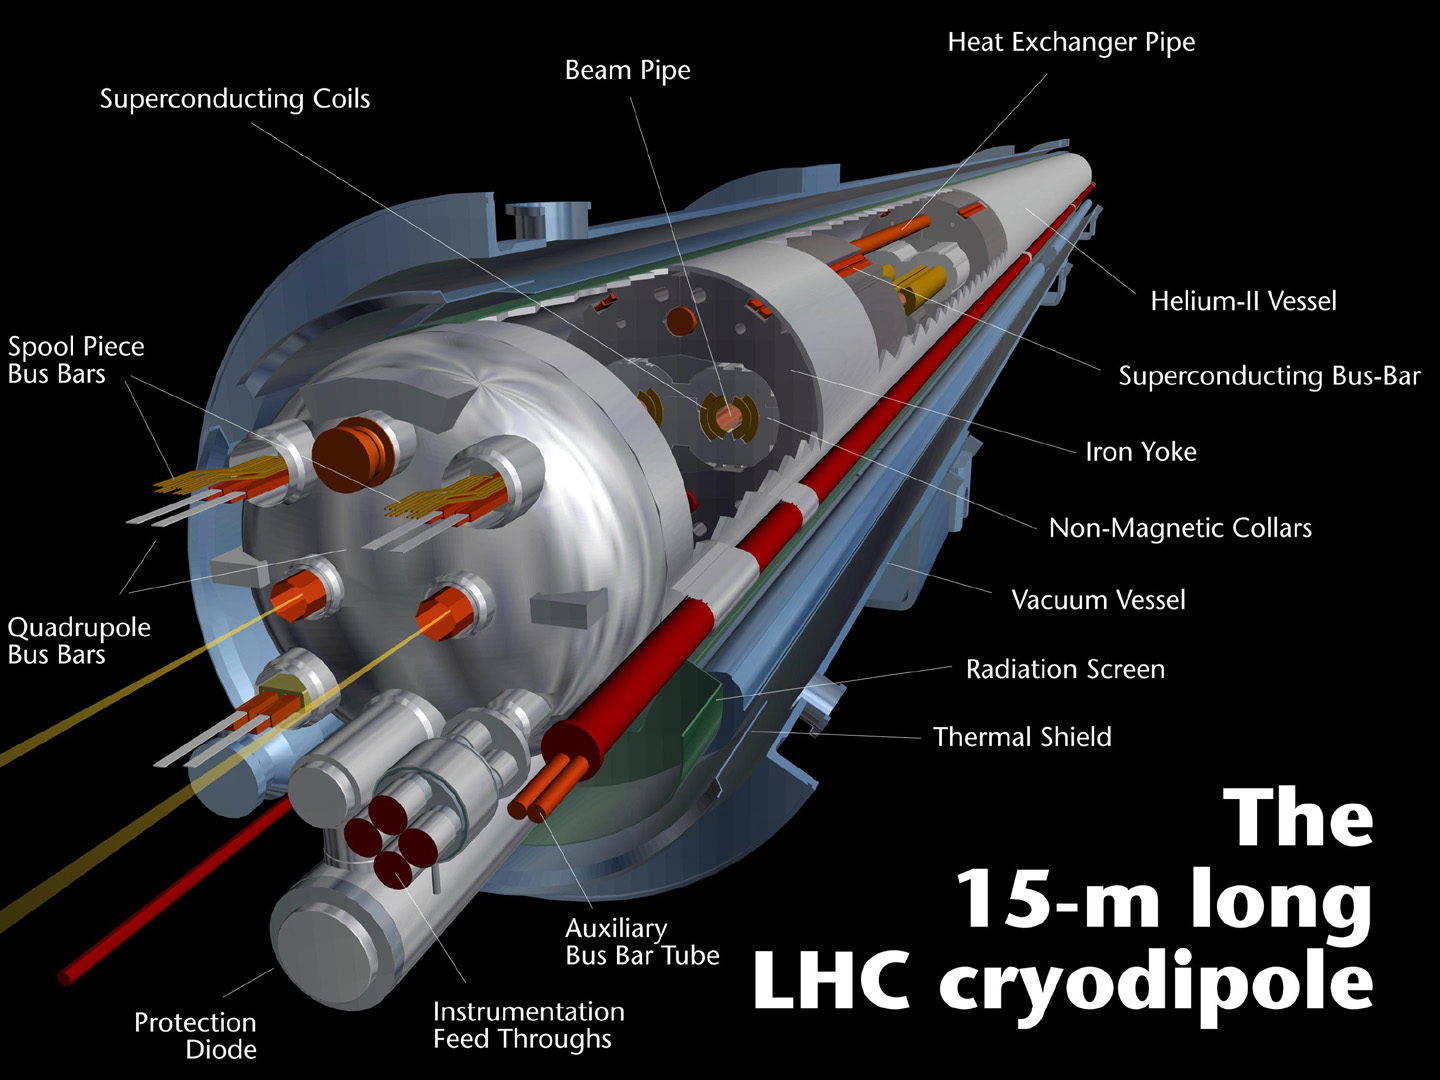
\includegraphics[width=0.9\textwidth]{figures/cryodipole.jpg} 
\\
\vspace{1cm}
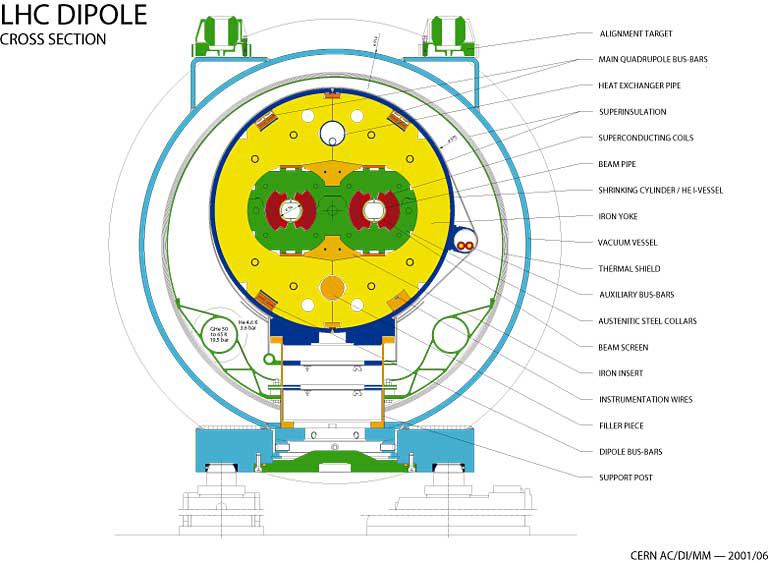
\includegraphics[width=0.45\textwidth]{figures/LHC-PHO-2001-187.jpg}
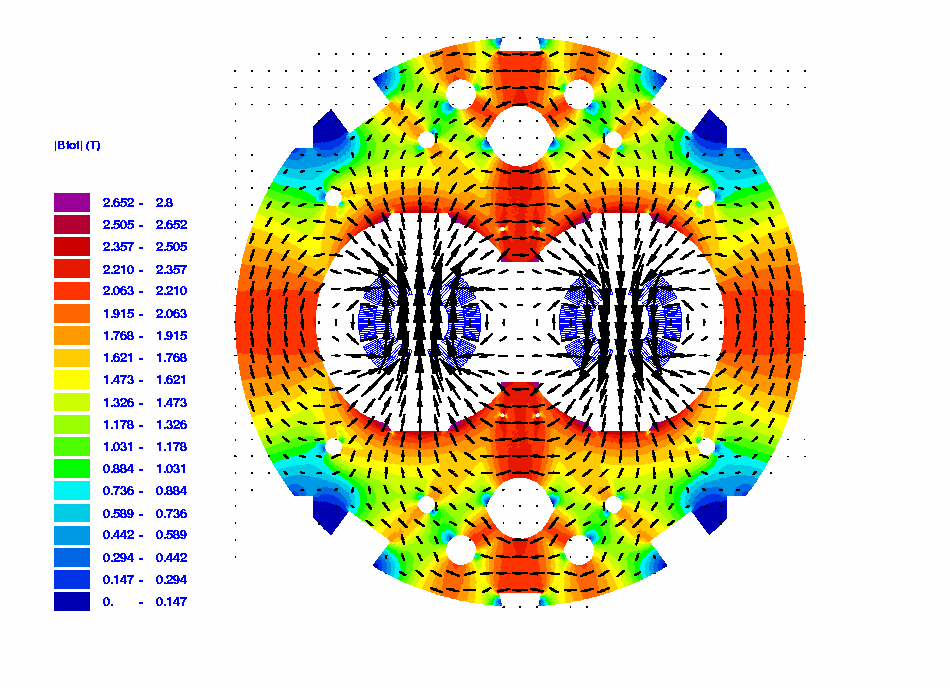
\includegraphics[width=0.45\textwidth]{figures/LHC-Dipole-Magnetic-Field.png}
\caption{The inner structure, cross section and magnetic field map of
an LHC cryodipole.} 
\label{fig:SCdipole} 
\end{figure} 

The luminosity is given by 
\begin{eqnarray} 
\mathcal{L} = \frac{\gamma f k_B N_p^2}{4 \pi \epsilon_n \beta^*} F 
\end{eqnarray} 
where $\gamma$ is the Lorentz factor, 
$f$ is the revolution frequency, 
$k_B$ is the number of bunches,
$N_p$ is the number of protons per bunch, 
$\epsilon_n$ is the normalized transverse emittance, 
$\beta^*$ the amplitude function at the interaction point, 
and $F$ is the reduction factor due to the crossing angle.
The left figure in fig.~\ref{fig:intlumi} shows the integrated luminosity 
delivered by LHC in 2010, 2011 and 2012 as a function of time each year. 
The delivered intgrated luminosity is 6.1~\ifb\ at $\sqrt{s}=7~\TeV$ in 2011
and 23.3~\ifb\ at $\sqrt{s}=8~\TeV$ in 2012. 

While a perfect detector can record the delivered luminostiy 
with 100~\% efficiency, in reality there are lost collisions 
due data aquisition system being busy and temparary unavailability 
of detector subsystems.  
The right figure in fig.~\ref{fig:intlumi} shows the delivered and the recorded luminosity 
integrated in the 2012 run period. Of the 23.30~\ifb of the delivered luminosity,  
21.79~\ifb is recorded by CMS detector.  

%
\begin{figure}[ht!] 
\centering 
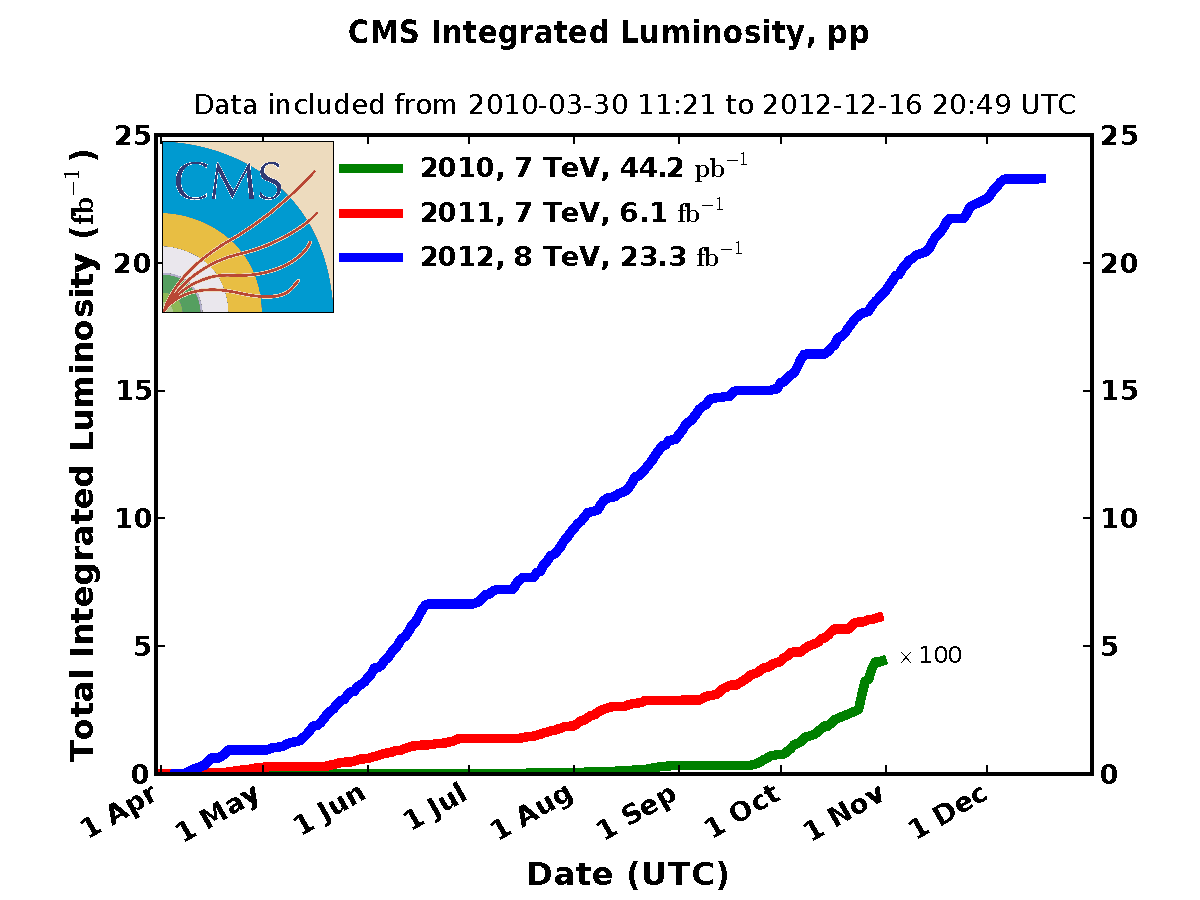
\includegraphics[width=0.45\textwidth]{figures/int_lumi_cumulative_pp_2.pdf}
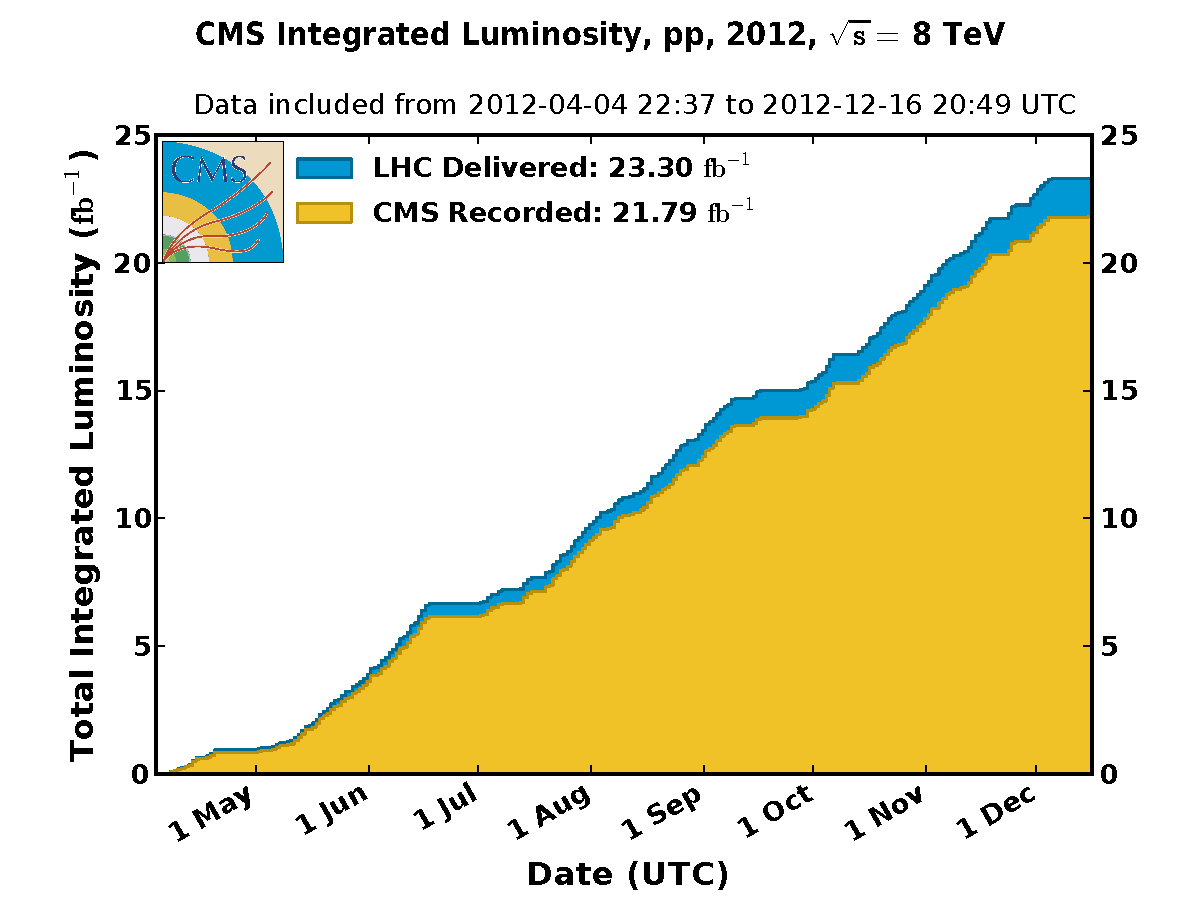
\includegraphics[width=0.45\textwidth]{figures/int_lumi_per_day_cumulative_pp_2012.pdf}
\caption{Integrated luminosity delivered by LHC in 2010, 2011 and 2012 on left. 
Integrated luminosity delivered by LHC and recored by CMS in 2012 on right.} 
\label{fig:intlumi} 
\end{figure} 

As the proton beams are very squeezed in a proton bunch, there are multiple 
proton-to-proton interactions in one bunch crossing. This multiple interaction 
is called PileUp. The PileUp can be calculated by 
\begin{eqnarray} 
N_\textrm{{PU}} 
= 
\sigma_{\textrm{min bias}} \times \mathcal{L}_{\textrm{bunch crossing}} 
\end{eqnarray} 
where $N_{PU}$ is the number of PileUp events, 
$\sigma_{\textrm{min bias}}$ is the inelastic p-p cross section, 
and $\mathcal{L}_{bunch crossing}$ is the luminosity per bunch crossing.
In 2011 and 2012 the proton bunches crossed every 50~ns 
and the pick instantaneous luminosity is $7.7\times 10^{33} ~\cm^{-2}\textrm{s}^{-1}$. 
Fig.~\ref{fig:pileup2012} shows the PileUp distribution 
of the data recored by CMS detector in 2012 run period. 
The average PileUp is 21. 


%
\begin{figure}[ht!] 
\centering 
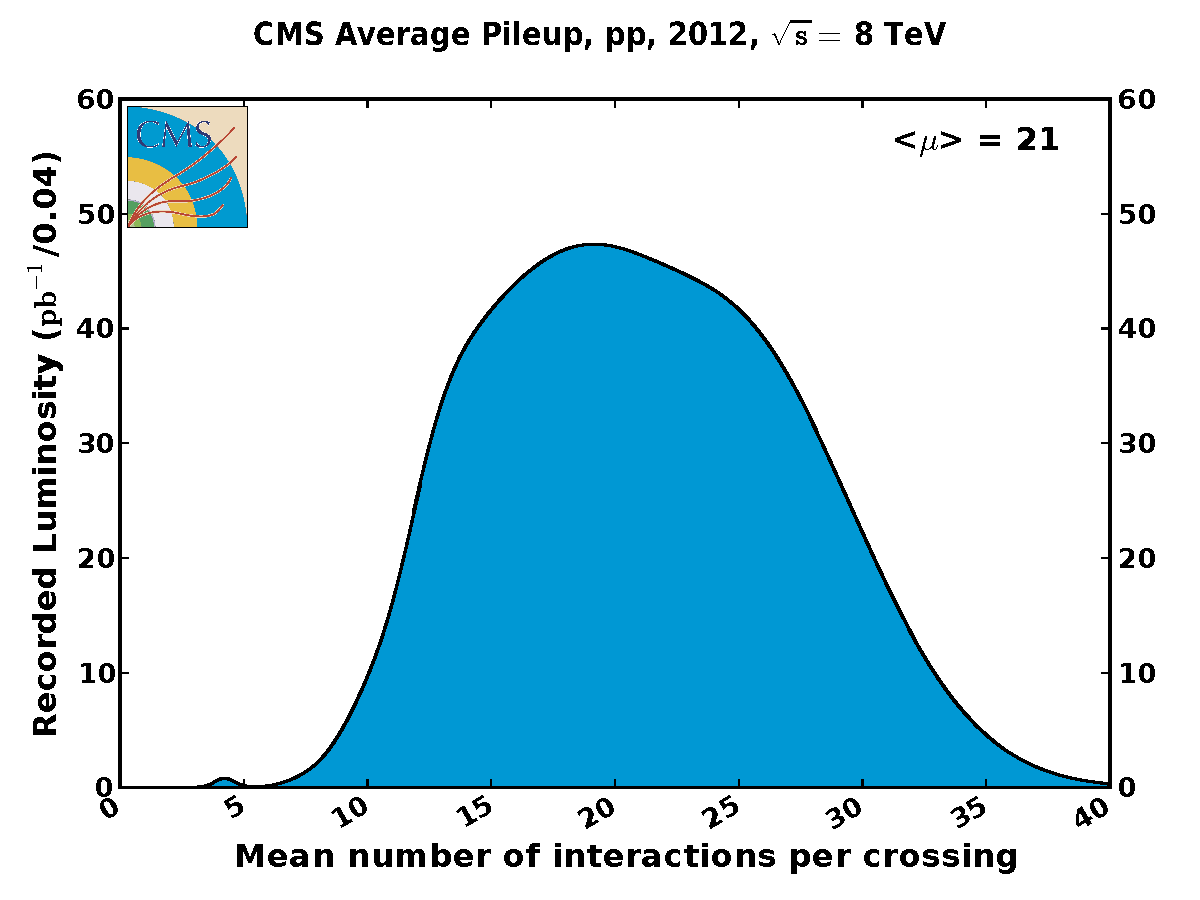
\includegraphics[width=0.7\textwidth]{figures/pileup_pp_2012.pdf}
\caption{Number of interactions per bunch crossing in 2012 run period.} 
\label{fig:pileup2012} 
\end{figure} 


\section{Compact Muon Solenoid detector} 

%\begin{itemize} 
%\item Design concept : target physics process 
%\item Coordinate convention : xyz axes, $\phi$, $\eta$, ...
%\item Discuss only hardware aspects(purpose of each detector, motivation of design, geometry, specification, electronics, performance ...)
%\end{itemize} 

There are two multi-purpose detectors built at the points where 
the two beams collide. Compact Muon Solenoid(CMS) detector~\cite{cmstdr1} is one of them. 
The design of the CMS detector is based on the the detection of SM Higgs boson
in the wide mass range, especially, $H \rightarrow \gamma\gamma$ in the low \mHi\ range 
and $H \rightarrow ZZ \rightarrow 4l$ in the medium \mHi\ range. 
To achieve this the detector need to have good muon identification and momentum resolution, 
good charged particle momeumtum resolution and reconstruction efficiency, 
good electromagnetic energy resolution, and good \met\ and di-jet mass resolution. 
The design of the CMS detector described in the following secions 
is to meet these requirements. 

The momentum and location of physics objects is expressed with respect to the origin 
centered at the collision point in the detector. The x-axis points to the center 
of the collider, the y-axis points upward, and the z-axis goes clock-wise along the 
beam line. CMS uses cylinderical coordinate system due to its cylinderical shape. 
The azimuthal angle, $\phi$, is the angle in the x-y plane 
and the polar angle, $\theta$, is measured with respect to the z-axis. 
Pseudorapidity is defined as $\eta = - \ln \tan(\theta/2)$. 
Advantage of pseudorapidity is that its difference is Lorentz invariant 
under longitidinal boost \footnote[1]{  
In frame O, 
\begin{equation} 
y_1 = \frac{1}{2} \ln \frac{E_1+p_{1L}}{E_1-p_{1L}} \textrm{ and } 
y_2 = \frac{1}{2} \ln \frac{E_2+p_{2L}}{E_2-p_{2L}}  
\end{equation} 
\begin{equation} 
\triangle y = y_1 - y_2 = \frac{1}{2} 
  \ln \frac{(E_1+p_{1L})(E_2-p_{2L})}{(E_1-p_{1L})(E_2+p_{2L})} 
\end{equation} 
In frame O' which is boosted to z direction with velocity $\beta = v / c$, 
\begin{equation} 
\triangle y' = y_1' - y_2' =  \frac{1}{2} 
  \ln \frac{(E_1'+p_{1L}')(E_2'-p_{2L}')}{(E_1'-p_{1L}')(E_2'+p_{2L}')} 
\end{equation}
where 
\begin{equation} 
E_i' = \gamma(E_i - \beta p_i) \textrm{ and } p_i' = \gamma(-\beta E_i + p_i)
\quad \quad \quad \quad (i = 1, 2)
\end{equation} 
Thus we have 
\begin{eqnarray} 
\triangle y' 
 &=& 
 \frac{1}{2} 
  \ln \frac{( \gamma(E_1 - \beta p_{1L})+\gamma(-\beta E_1 + p_{1L})')
            ( \gamma(E_2 - \beta p_{2L})-\gamma(-\beta E_2 + p_{2L}))}
           {( \gamma(E_1 - \beta p_{1L})-\gamma(-\beta E_1 + p_{1L}))
            ( \gamma(E_2 - \beta p_{2L})+\gamma(-\beta E_2 + p_{2L}))}  \\
 &=& 
 \frac{1}{2} 
  \ln \frac{ (E_1+p_{1L})(1-\beta)((E_2-p_{2L})(1+\beta) }
           { (E_1-p_{1L})(1+\beta)((E_2+p_{2L})(1-\beta) } \\ 
 &=& 
 \frac{1}{2} 
  \ln \frac{ (E_1+p_{1L})(E_2-p_{2L}) }
           { (E_1-p_{1L})(E_2+p_{2L}) } \\ 
 &=& \triangle y
\end{eqnarray} 
The rapidity difference is invariant under Lorentz boost along the beam axis. 
}.
Because the initial momentum in z direction is not known due to movement of 
partons inside a proton, and momentum x and y direction is almost zero, 
the momentum and energy of an object is expressed in terms of 
transverse quantitites, \pt\ and $E_T$, calculated in the transverse plane using 
only x and y components.

The overall layout of the CMS detector is as follows. 
Starting from the collision point to outward, there is the inner tracker system(Tracker) 
that is composed of pixel detector and silicon strips and covers $|\eta|<2.5$, 
Electromagnetic calorimeter(ECAL) that covers  $|\eta|<3.0$, 
Hadronic calorimeter(HCAL) that covers  $|\eta|<5.0$, the magnet system, 
and the muon system that covers  $|\eta|<2.4$. 
%\textcolor{red}{... make this paragraph richer ... } 
The details of the each sub-detector system are described in the following sections. 



%The design of the CMS detector was driven to achieve good momentum resolution of muons. 
%This requires a strong magnetic field that allows a good momentum measurement 
%of charged particles. Thus, CMS uses superconduncting  


\subsection{Tracker}

The purpose of tracker is to measure momentum of charged particles. 
Based on the charged particle flux, the tracker volume can be divided 
into 3 regions in radial direction. The first region is $r<20~\cm$, closest 
to the interaction vertex. Due to highest particle flux, pixel detectors 
each of which has size of $100 \times 150~\um^2$ are installed. 
The occupancy is about $0.01$ \% per pixel per crossing. 
The second region is $20<r<55~\cm$ and the particle flux is low so that silicon 
microstrip detectors can be used. Minimum size of cell is $10~\cm \times 80~\um$.
The occupancy is about $2-3$ \% per pixel per crossing. 
The third region is $55<r<110~\cm$ and larger-pitch silicon microstrips
are used. The maximum size of a cell is $25~\cm \times 180~\um$.
The occupancy is about $1$ \% per pixel per crossing. 

The layout of the tracker is shown in fig.~\ref{fig:trackerlayout}. 
The total size is 1.1~m in radius and 5.4~m in length. 
In the barrel region, there 3 layers of hybrid pixel detectors
at r = 4.4, 7.3 and 10.2~\cm. The silicon microstrips are 
placed in $20<r<110~\cm$. The barrel region is further separated 
into Inner Barrel(TIB) with 4 layers and Outer Barrel(TOB) with 6 layers. 
In TIB there 3 Inner Disks(TID) in the transition region 
to avoid to small track crossing angle. 
In endcap region, there are 2 pixel and 9 microstrip layers. 
The tracker provides coverage, $|\eta|<2.5$.
%
\begin{figure}[htp] 
\centering 
\begin{tabular}{c} 
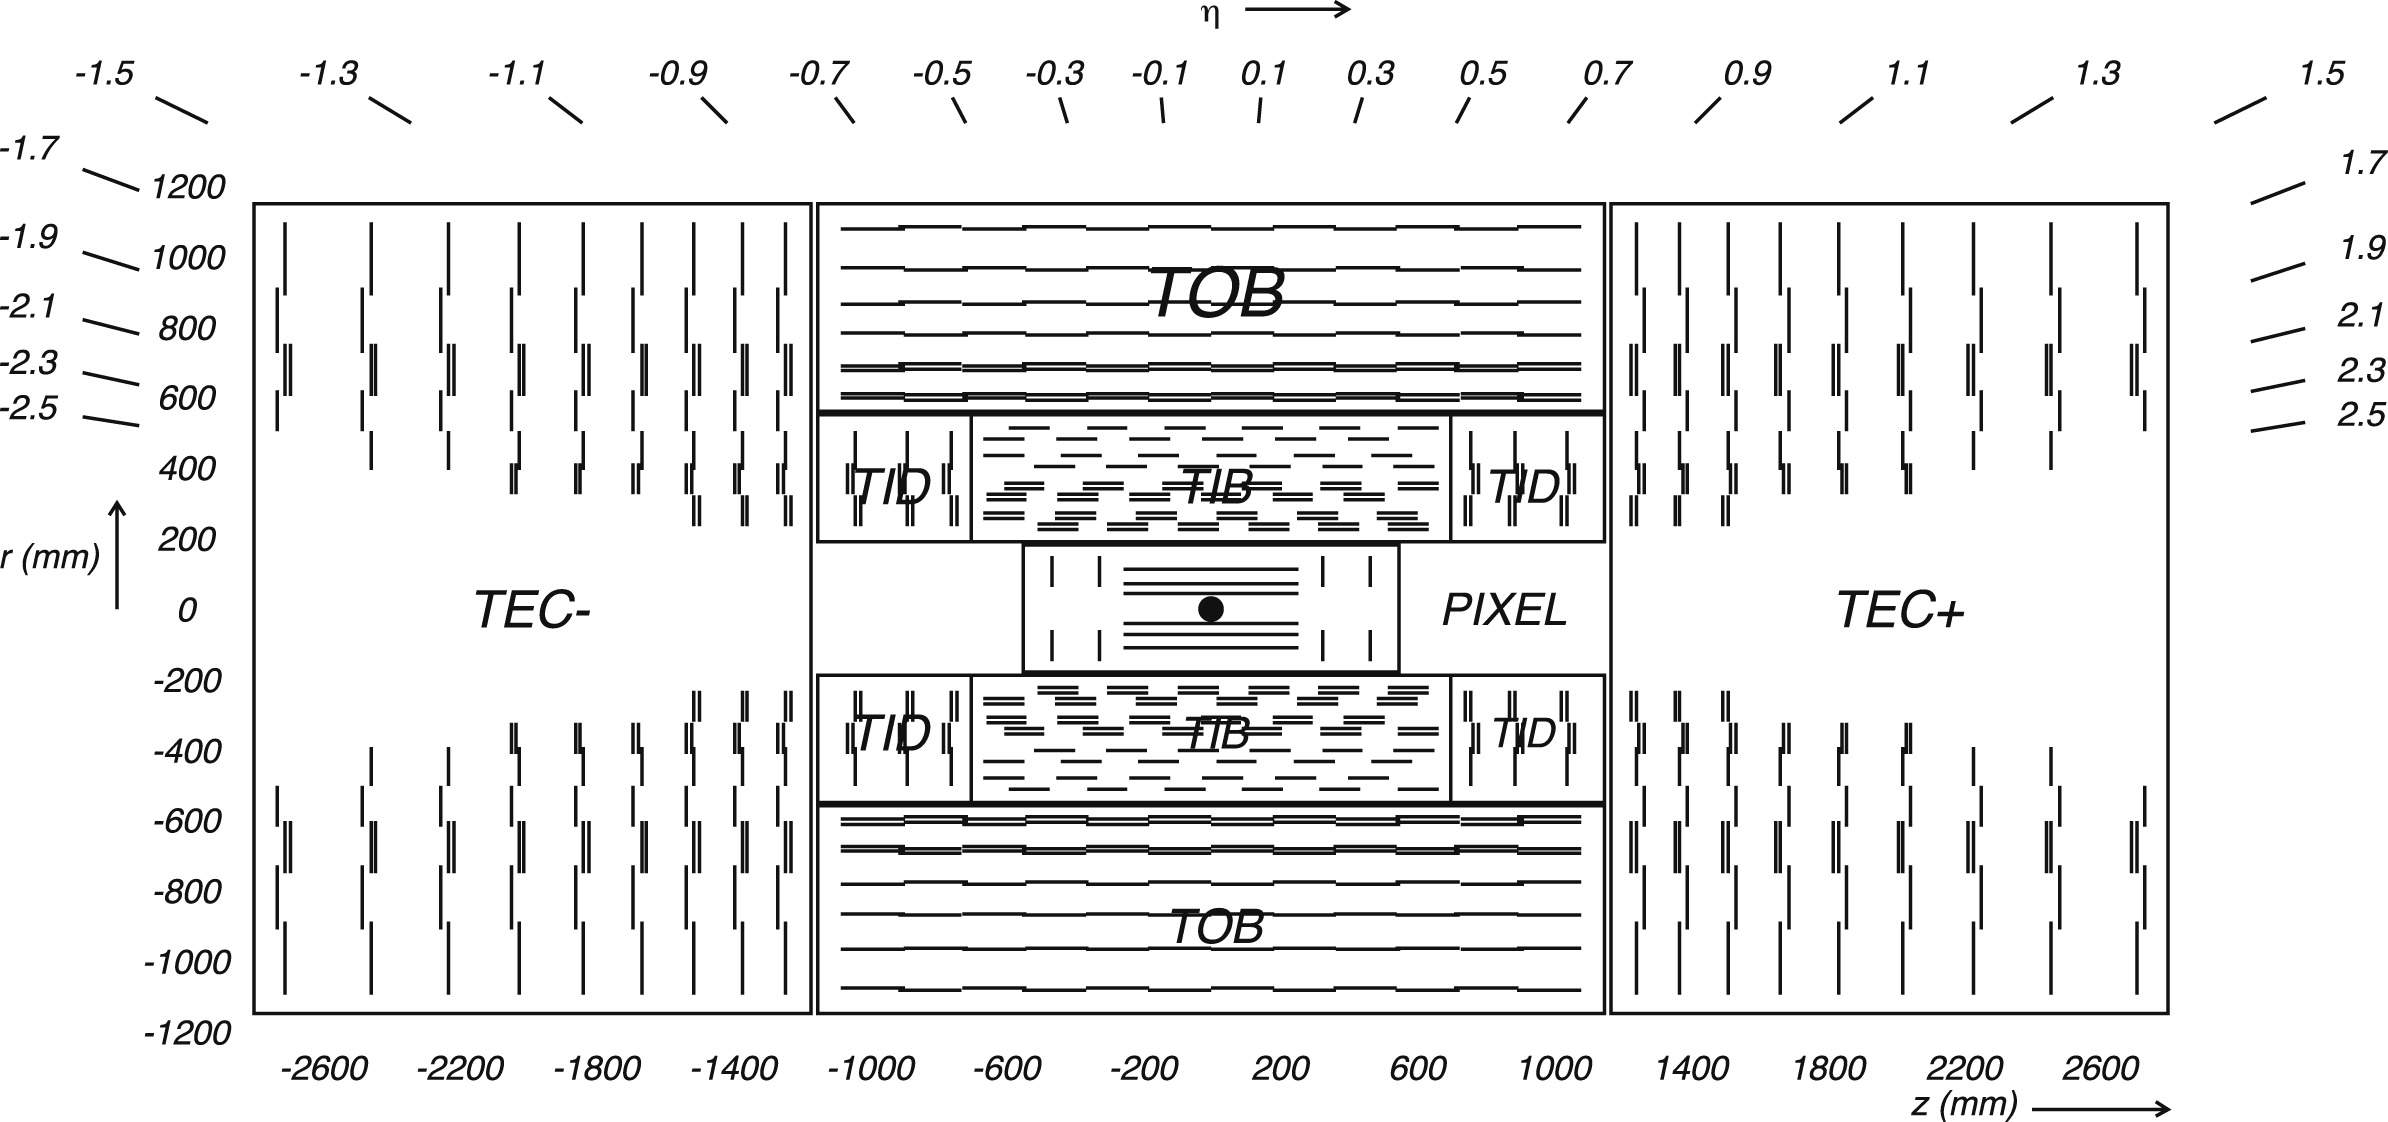
\includegraphics[width=0.99\textwidth]{figures/trackerlayout.jpeg} 
\end{tabular} 
\caption{The layout of the CMS tracker~\cite{Anghel2009277}.} 
\label{fig:trackerlayout} 
\end{figure} 

The pixel tracker is composed of 3 layers in barrel and 2 disks in both 
endcap region. The barrel layers are placed at r = 4.4, 7.3 and 10.2~\cm
and each of them has length 53~\cm. The endcap disks cover $6<r<15~\cm$
and located at $|z|=34.5~\cm$ and $46.5~\cm$. The dimension of each 
pixel is $100~\um$ in $r$ and $\phi$, and $150~\um^2$ in $z$.  
The size is chosen to take into account Lorentz drift  
% look at 1.2.1 of http://people.web.psi.ch/kotlinski/CMS/Varia/cmspixel.pdf
\footnote{
Charge carriers in the pixel detector are deflected by the magnetic field perpendicular 
to the electric field. }
and to maintain charge sharing between multiple pixels. 
Each endcap disk is composed of 24 blades assembled to form 
a turbine-like geometry and the blades are rotated by 20~\dg\
considering Lorentz effect. The pixel detector provides 
spatial resolution of 10 and 20~\um\ for $r-\phi$ and $z$ measurements, 
respectively.

The strip tracker is composed of TIB and TOB in barrel region
and TEC and TID in the endcap region. The Number of detectors, thickness,
and mean pitch is shown in the tab.~\ref{tab:silicondetectorspec}.
The first and the second layers of TIB are made with stereo modules
with angle 100~mrad providing single-point resolution of 23-34~\um\
in the $r-\phi$ direction and 230~\um\ in z direction. As TIB, the 
first and the second layers of TOB are made with stereo modules
with angle 100~mrad providing single-point resolution of 35-52~\um\
in the $r-\phi$ direction and 530~\um\ in z direction.
In the endcap region, the first and the second layers of TID, and the first, 
second and the fifth layers of TEC are stereo modules that provide. 
%
\begin{table}[htp] 
\begin{center} 
\small
\begin{tabular}{c|ccccc}  
\hline 
Part & Number of & thickness & mean pitch   & coverage & layers     \\ 
     & detectors & (\um)     & (\um)        &          & (disks)    \\ 
\hline \hline 
%TIB     & 2724  &   320     &   81/118          & $|z|<65~\cm$      & 4     \\ 
%TOB     & 5208  &   500     &   81/183          & $|z|<110~\cm$     & 6     \\ 
%TID     &  816  &   320     &   97/128/143      & $65<|z|<120~\cm$  & 3     \\ 
%TEC     & 2512  &   320     &   96/126/128/143  & $120<|z|<280~\cm$ & 9     \\ 
%TEC(2)  & 3888  &   500     &   143/158/183     &                   &       \\ 
TIB     & 2724  &   320     &   81-118          & $|z|<65~\cm$      & 4     \\ 
TOB     & 5208  &   500     &   81-183          & $|z|<110~\cm$     & 6     \\ 
TID     &  816  &   320     &   97-143          & $65<|z|<120~\cm$  & 3     \\ 
TEC     & 6400  &   320-500 &   96-183          & $120<|z|<280~\cm$ & 9     \\ 
\hline 
\end{tabular} 
\caption{Number of detectors, thickness and mean pitch of each strip, 
coverage in z direction, and number of layers(disks) of the four part of 
silicon strip detector, TIB, TOB, TID and TEC.} 
\label{tab:silicondetectorspec} 
\end{center} 
\end{table} 

Ideal tracker would have no energy loss of charged particles 
while they cross the tracker so that they deposit their initial 
energies in calorimeter. However, real trackers can not be made 
that way due to materials used to build the tracker such as 
electrical cables, cooling servies, support structures, 
electronics and beam-pipe. Fig.~\ref{fig:trackermaterial} shows 
the materal budget of tracker in the units of radiation length($X_0$) 
and interaction length($\lambda_0$). 
%
\begin{figure}[ht!] 
\vspace{1cm}
\centering 
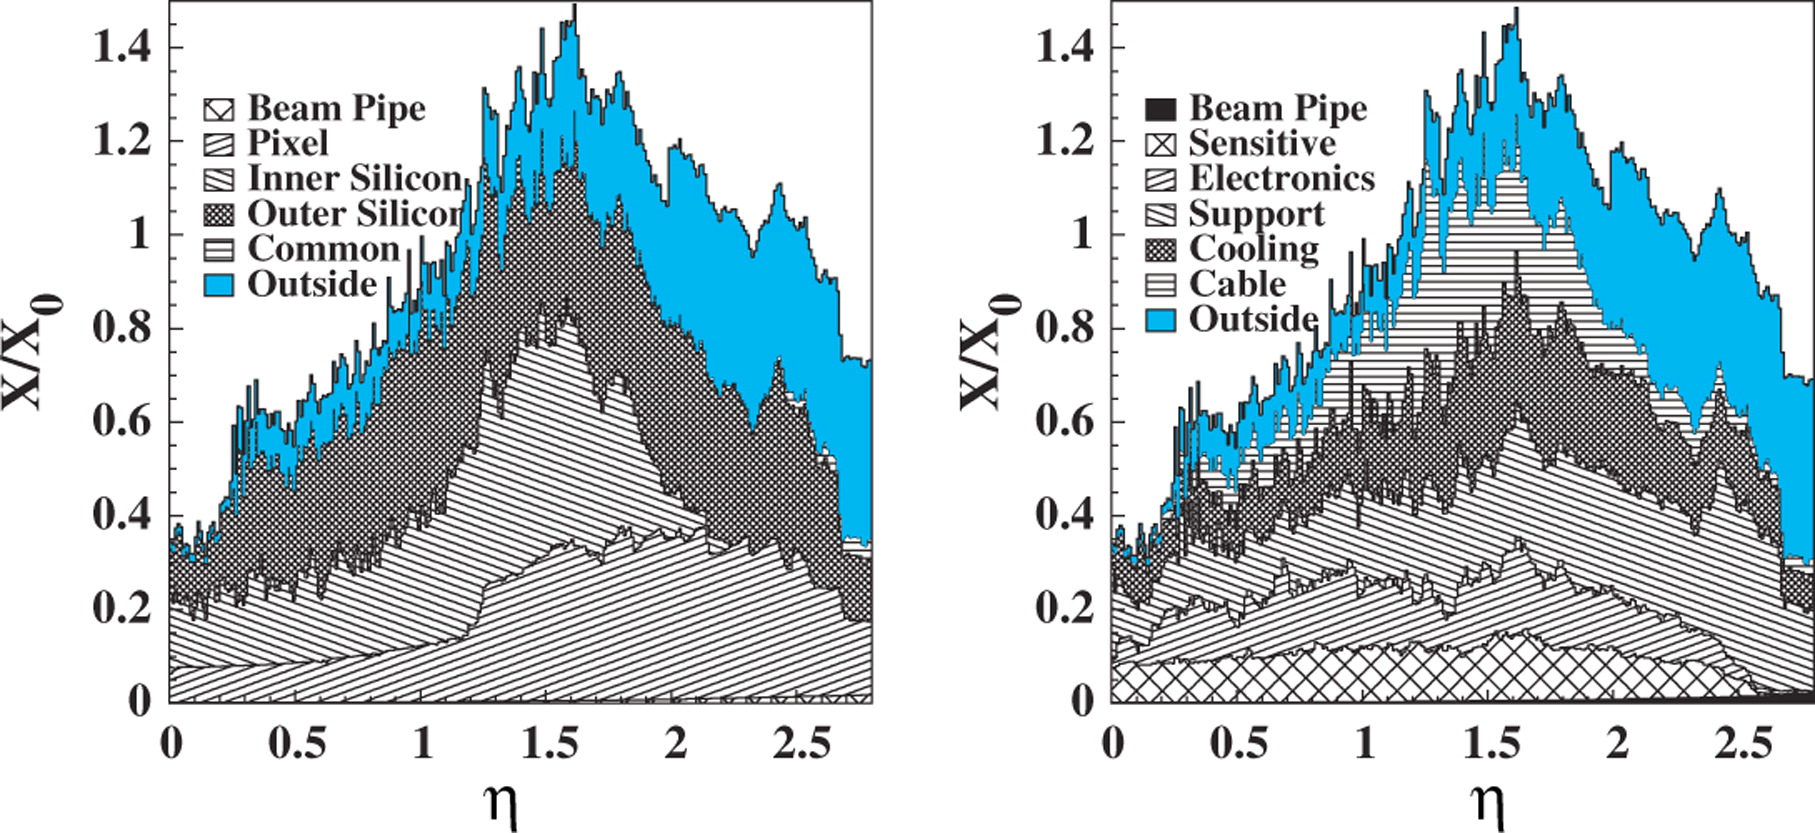
\includegraphics[width=0.99\textwidth]{figures/trackermaterial.jpeg}
\caption{Material budget of CMS tracker in terms of radiation length($X_0$)
and interaction length($\lambda_0$)~\cite{Abbaneo2004331}.} 
\label{fig:trackermaterial} 
\end{figure} 



%%%%%%%%
\subsection{Electromagnetic Calorimeter} 
%\begin{itemize}
%  \item Selective readout   
%  \item Performance  
%\end{itemize}

The Electromagnetic Calorimeter(ECAL) is crucial to measure the energy 
of electrons and photons. The CMS ECAL is composed of 61200 and 7324 
lead tunstate($\textrm{PbWO}_4$) scintilating crystals in barrel and 
endcap regions, repectively. $\textrm{PbWO}_4$ crystals have short 
radination length(0.89~\cm) and small Molirere radius(2.2~\cm). 
It is fast in emitting lights and radiation resistant. 
But, it produces relatively low light yields, which requires amplification 
of light signal using photodetectors. Silicon avalanche photodiondes(APD)
are used in barrel and vacuum pohtontriodes(VPT) are used in endcap.
The crystals and APDs are sensitivie with temperature, so the stability
of temperautre is required for operation of ECAL. 

In the barrel region(EB), there are 36 supermodules and each covers 
the region, $0 < |\eta| < 1.479$. 
As shown in fig.~\ref{fig:ecal_EB}, one supermodule contains 4 modules 
and each module has 40 - 50 submodules 
which are composed of 10($2 \times 5$) sub-units(one crystal + one capsule). 
Each crystal covers $0.0174 \times 0.0174$($\approx 1~\dg \times 1~\dg$)
in $\Delta \phi \times \Delta \eta$ and is tilted at 3~\dg\ with respect to the line 
from nominal vertex position. %\textcolor{red}{why tilted?}
The length of a crystal is 230~\mm\ which corresponds to $25.8X_0$.
%http://zitogiuseppe.com/oldf/pguide.html

In the endcap region(EE) as shown in fig.~\ref{fig:ecal_EE}, 
the basic unit is supercrystal which is a collection of $5 \times 5$ crystals. 
Each endcap regions is covered 
by two D-shape structred by supercrystals. 
One crystal has the front face size of $28.6 \times 28.6~\mm^2$ 
and length of 220~\mm($24.7X_0$).
Each crystal is off-pointing the nominal vertex as the barrel crystals.  
In the endcap region, the angle between the decayed photons 
is smaller than the barrel region, so an additional deviced is 
needed to distinguish the converted photons from genuine photons.
In order to do this, a preshower device is placed in front of the endcap crystals. 
The preshower device is made of 2 planes of silicon strip detectors with a pitch of 1.9~\mm\
behind disks of lead absorber of depth 2$X_0$ and 3$X_0$.
Due to its finer structure, it provides better spacial resolution 
that enables to reject false photons.  
% preshower : http://cms.web.cern.ch/news/ecal-preshower

%
\begin{figure}[h] 
\vspace{1cm}
\centering 
\begin{tabular}{|c|} 
\hline
\\
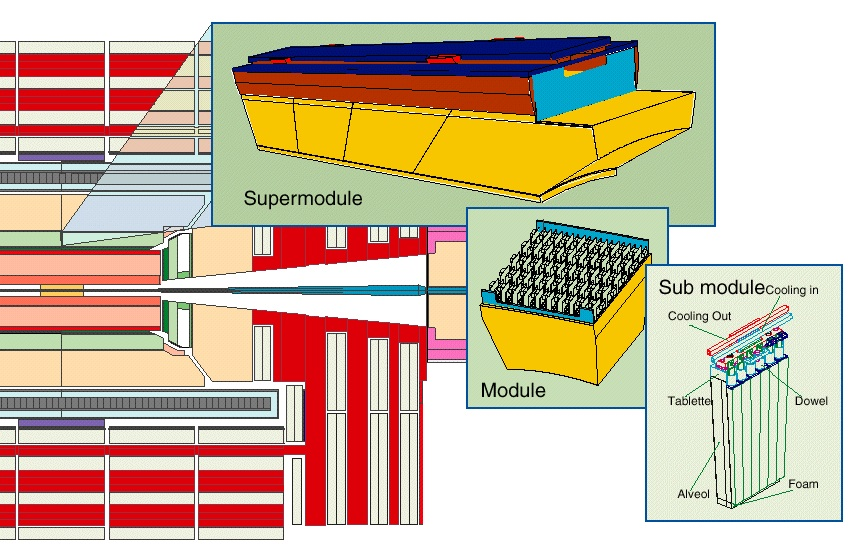
\includegraphics[width=0.8\textwidth]{figures/ecal_barrel.jpg} \\
\hline
\end{tabular} 
\caption{Barrel region of ECAL.}
\label{fig:ecal_EB} 
\end{figure} 
%
\begin{figure}[h] 
\vspace{1cm}
\centering 
\begin{tabular}{|c|} 
\hline
\\
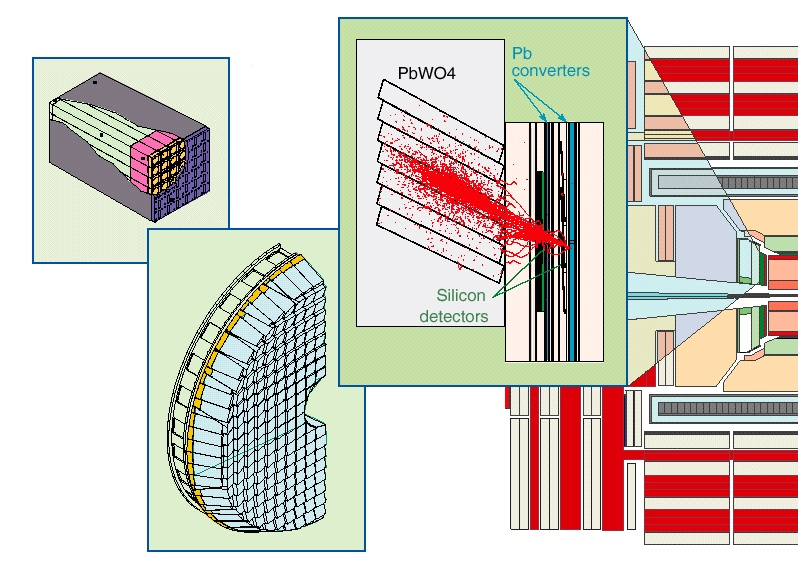
\includegraphics[width=0.8\textwidth]{figures/ecal_endcap.jpg} \\
\hline
\end{tabular} 
\caption{Endcap region of ECAL.}
\label{fig:ecal_EE} 
\end{figure} 
%
%\begin{figure}[ht!] 
%\vspace{1cm}
%\centering 
%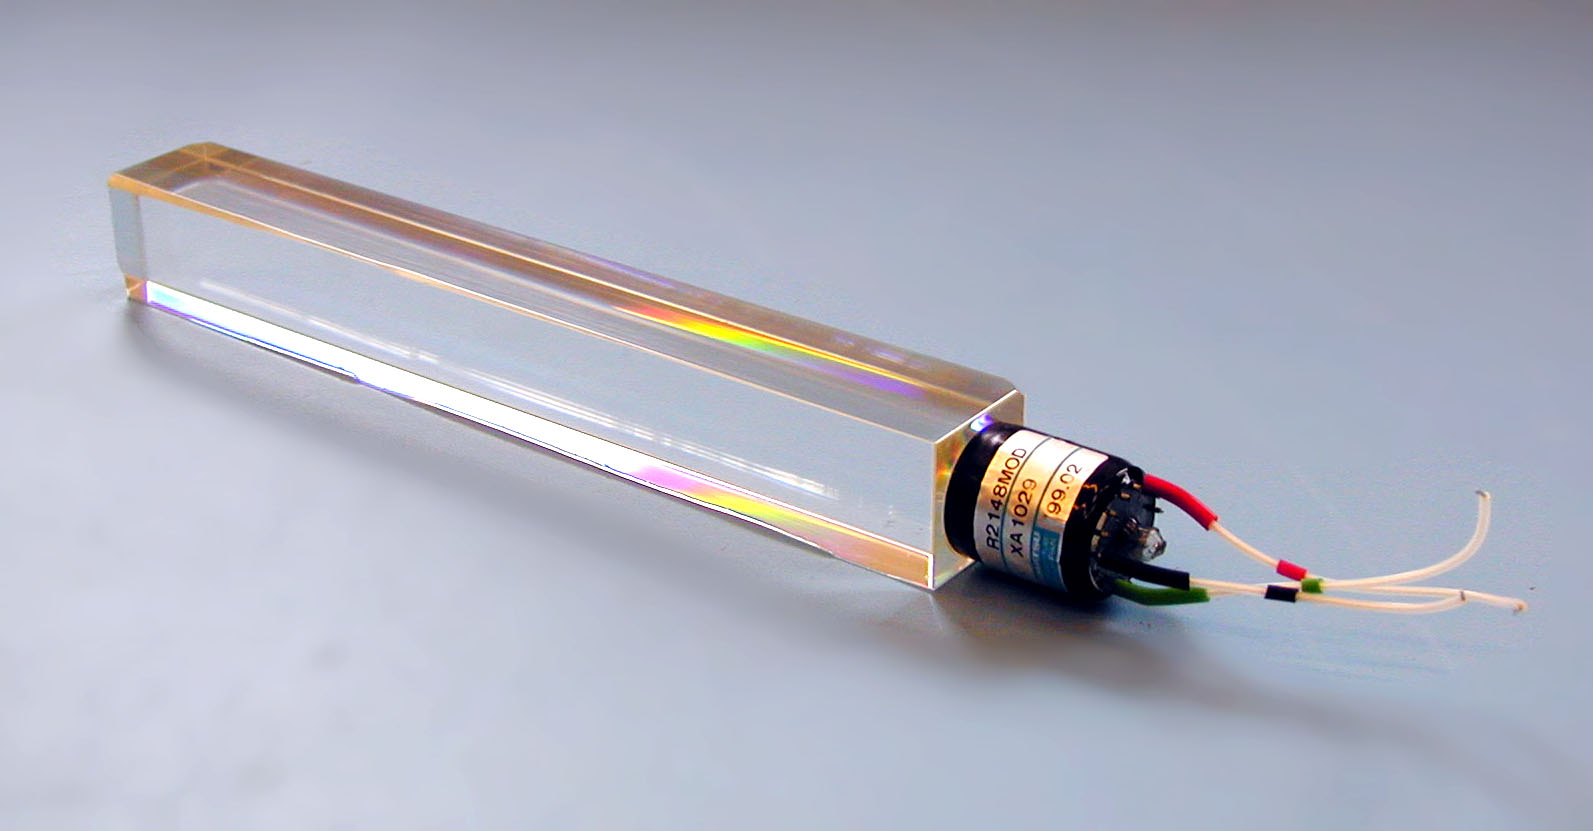
\includegraphics[width=0.99\textwidth]{figures/EE_Crystal.jpg}
%\caption{Endcap crystal and VPT.}
%\label{fig:EE_crystal} 
%\end{figure} 

The performance of the supermodule in the barrel region is measured 
using a test beam. The electrons in the test beam were indicient on 
the central crystal of $3\times 3$ crystals.
Fig.~\ref{fig:ecal_res} shows its energy resolution($\sigma(E)/E$)
as a function of beam energy(E). The eneryg resolution of calorimeters is 
parametrized by 
\begin{eqnarray}
\left( \frac{\sigma}{E} \right)^2 
= 
\left( \frac{S}{\sqrt{E}}  \right)^2 + \left( \frac{N}{E} \right)^2 + C^2
\end{eqnarray} 
where S is the stochastic term that reflects the fact that the development of showers is    
a statistical process, N is to account for instrumental effects such as noise and pedestals, 
and C is the constant term for calibration errors such as non-uniformitity of detectors.  
The figure shows corresponding values for two curves that use different trigger 
conditions. 

%
\begin{figure}[h] 
\vspace{1cm}
\centering 
\begin{tabular}{|c|} 
\hline
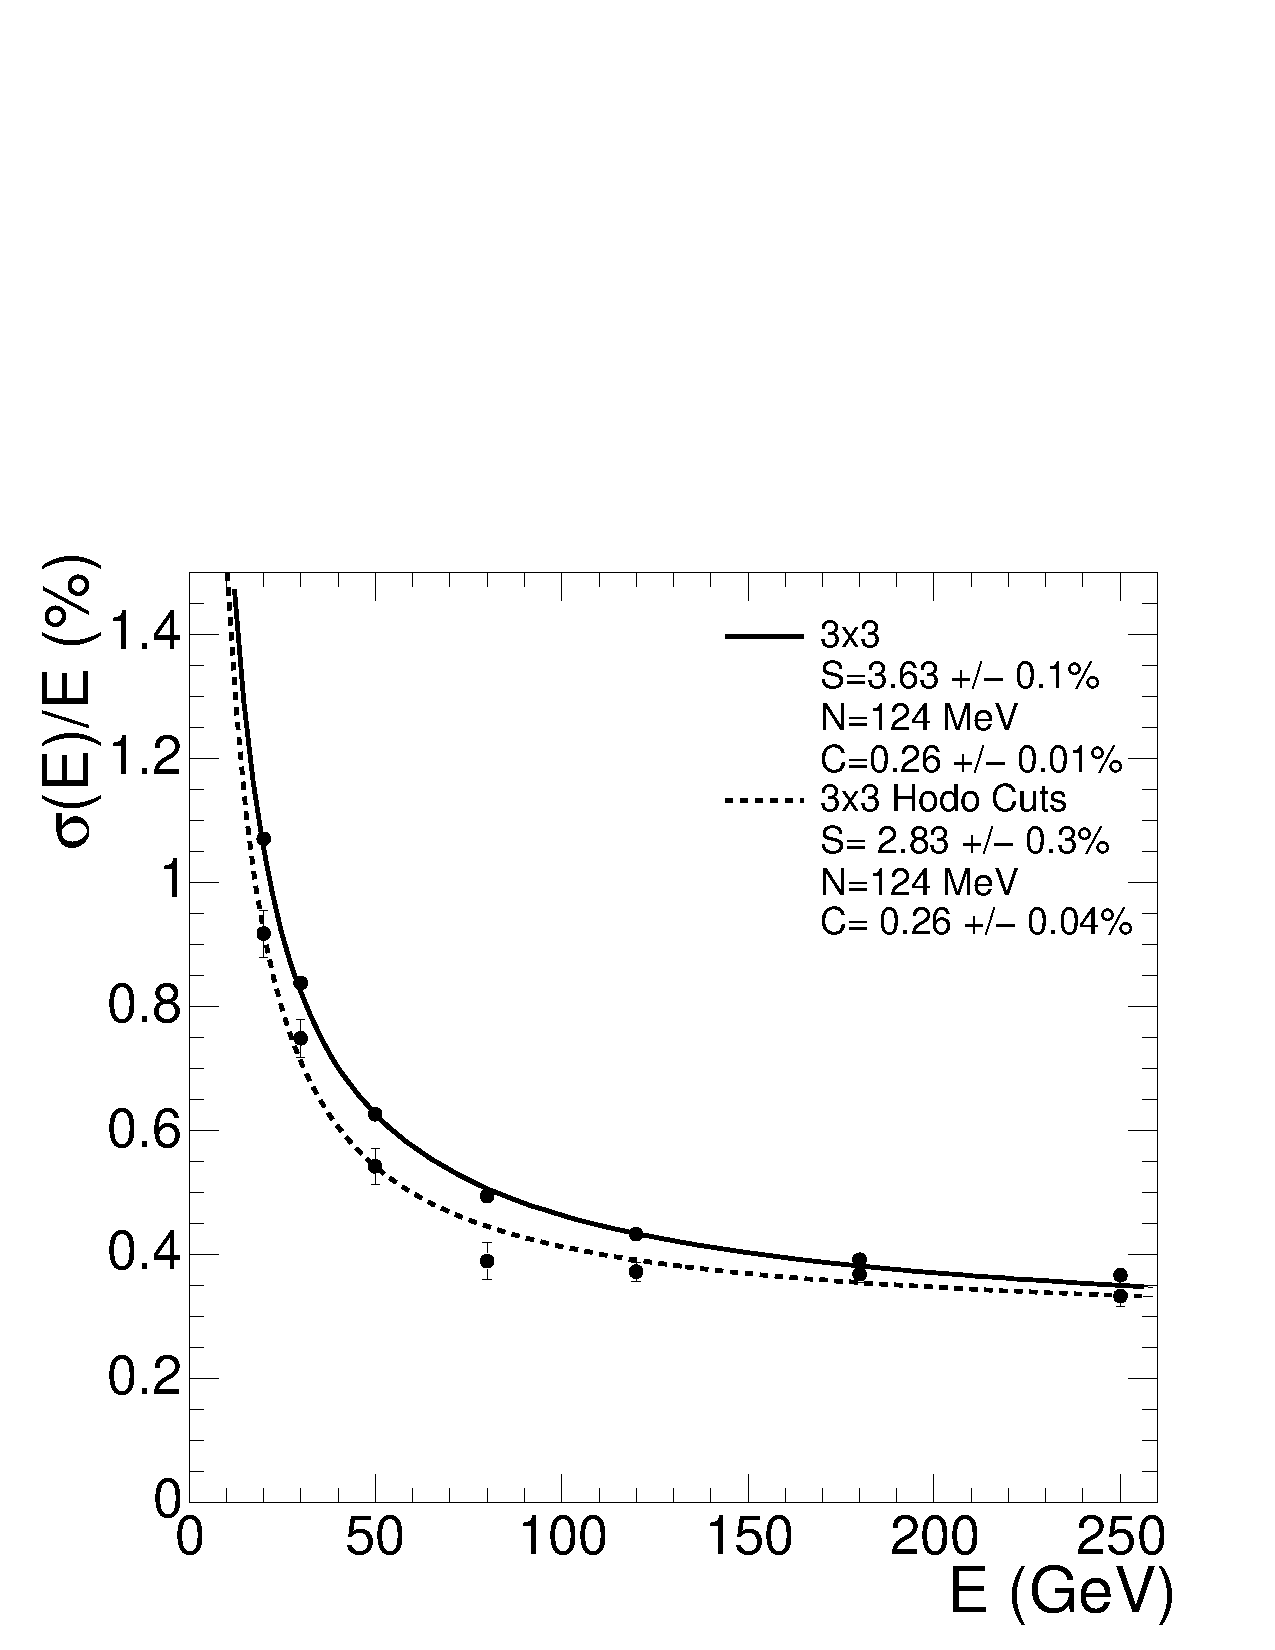
\includegraphics[width=0.6\textwidth]{figures/Figure_001-007.pdf}\\
\hline
\end{tabular} 
\caption{Energy resolution of ECAL supermodule measured using a test beam~\cite{cmstdr1}.}
\label{fig:ecal_res} 
\end{figure} 


%%%%%%%%
\subsection{Hadronic Calorimeter} 

The hadronic calorimeter(HCAL) is made to measure energy of jets.
For the design of HCAL it is important to minimize the Gaussian tails in the energy 
resolution, and to achieve good containment of energy desposit and 
hermeticity for \met\ calculation. CMS HCAL is a sampling detector 
that is composed of alternating layers of an absorber and a scintillator. 
As a hadronic particle hits an absorber plate, interactions occur to produce 
secondary particles, and the these produced particles interact with 
the material in the next layer of absorber, resulting in a shower of 
hadronic particles. When these particles cross the active scintillating  
layers, they cause them to emit lights which can be detected by 
optic devices. The choice of strong magnetic field made most of the 
HCAL built inside of the magnetic coils. This constrained to choose 
a material with short interaction length. For this reason, brass 
is chosen as the HCAL material. The CMS HCAL is organized to 
Hadron Barrel(HB), Hadron Outer(HO), Hadron Endcap(HE) and Hadron Forward(HF).  
Fig.~\ref{fig:hcal_layout} shows the layout of CMS HCAL where HF is not shown. 
%
\begin{figure}[h] 
\vspace{1cm}
\centering 
\begin{tabular}{|c|} 
\hline
\\
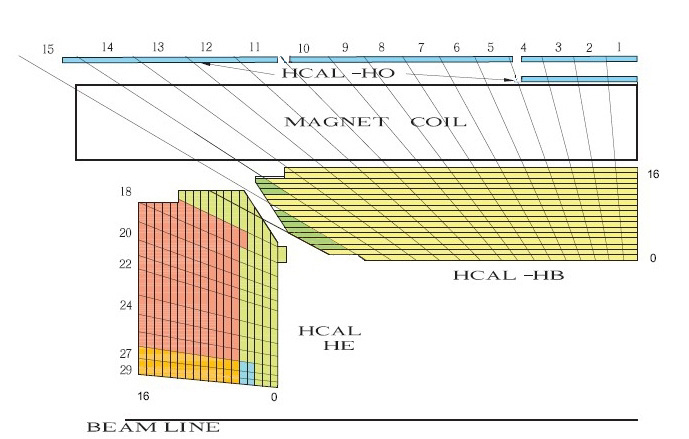
\includegraphics[width=0.99\textwidth]{figures/Hcal-segementation-updated.JPG}\\
\hline
\end{tabular} 
\caption{Layout of CMS HCAL~\cite{Chatrchyan:2009hw}.}
\label{fig:hcal_layout} 
\end{figure} 

HB consists of 2304($32 \times 72$ in $\eta \times \phi$) towers of size 
$\Delta \phi \times \Delta \eta = 0.087 \times 0.087$. One HCAL tower 
has the same $\Delta \phi \times \Delta \eta$ coverage as $5\times5$
ECAL crystals. There are 15 brass plates with thickness 5~\cm\ and 
2 stainless steel for mechanical support. The first scintillating 
plate placed before the first brass plate has width of 9~\mm\ while 
the other 16 scintillating plates have width of 3.7~\mm. 

In the barrel, HO which covers $|\eta|<1.26$ is placed to complement 
the short length of HB that may not be enough 
to contain all particles. The escaping showering particles 
is the cause of tail in the energy resolution. Adding HO effectively increases 
the interaction length over 10, thus energy resolution is enhanced.
This is very important for \met\ resolution calculated using calorimeter information. 
HO is divided into 5 sections in $\eta$, resulting 5 rings 
each of which covers 2.5~m in z direction. 
The central ring has two layers of scintillator placed at $r=3.85~\textrm{m}$ and 
$r=4.097~\textrm{m}$ with an iron absorber of thickness 18~\cm\ between them. 
The other rings have one scintillator layer at $r=4.097~\textrm{m}$.

HE is composed of 2304 towers covering $1.3 < |\eta| < 3.0$. 
As shown in left figure of fig.~\ref{fig:hcal_HEHF}, the 5 othermost towers have 
$\phi$ segmentation of 5~\dg\ and $\eta$ segmentation of 0.087. 
The 8 innermost towers have 
$\phi$ segmentation of 10~\dg\ and varying $\eta$ segmentations of 0.09 - 0.35. 

HF is located at $z = \pm 11.2~\textrm{m}$ covering $3.0 < |\eta| < 5.0$. 
It provides improvement in measurement of \met\ 
and reconstruction of forward jets which can be used to identify very interesting 
processes such as Vectro Boson Fusion(VBF).%~\cite{}. 
Because HF receive the bulk of particle energy of the collision, 
the material should be resitive to radition. 
HF moduels are made of steel blocks with quartz fibers.
The particles crossing the fibers emit Cherenkov lights 
and the lights are collected by photomultipliers connected to 
the fibers. The right figure of fig.~\ref{fig:hcal_HEHF} shows 
a $\Delta \phi=20~\dg$ wedge of HF.  
The $\phi$ segmentation is 10~\dg\ for all towers except for the 
the two innersmost towers which have $\Delta \phi=$20~\dg. 
The $\eta$ segmentation is 0.175 except for the innermost 
and the outermost towers which have $\Delta \eta=$ 0.3 and 0.1, respectivley. 
%
\begin{figure}[h] 
\vspace{1cm}
\centering 
\begin{tabular}{cc} 
%\hline
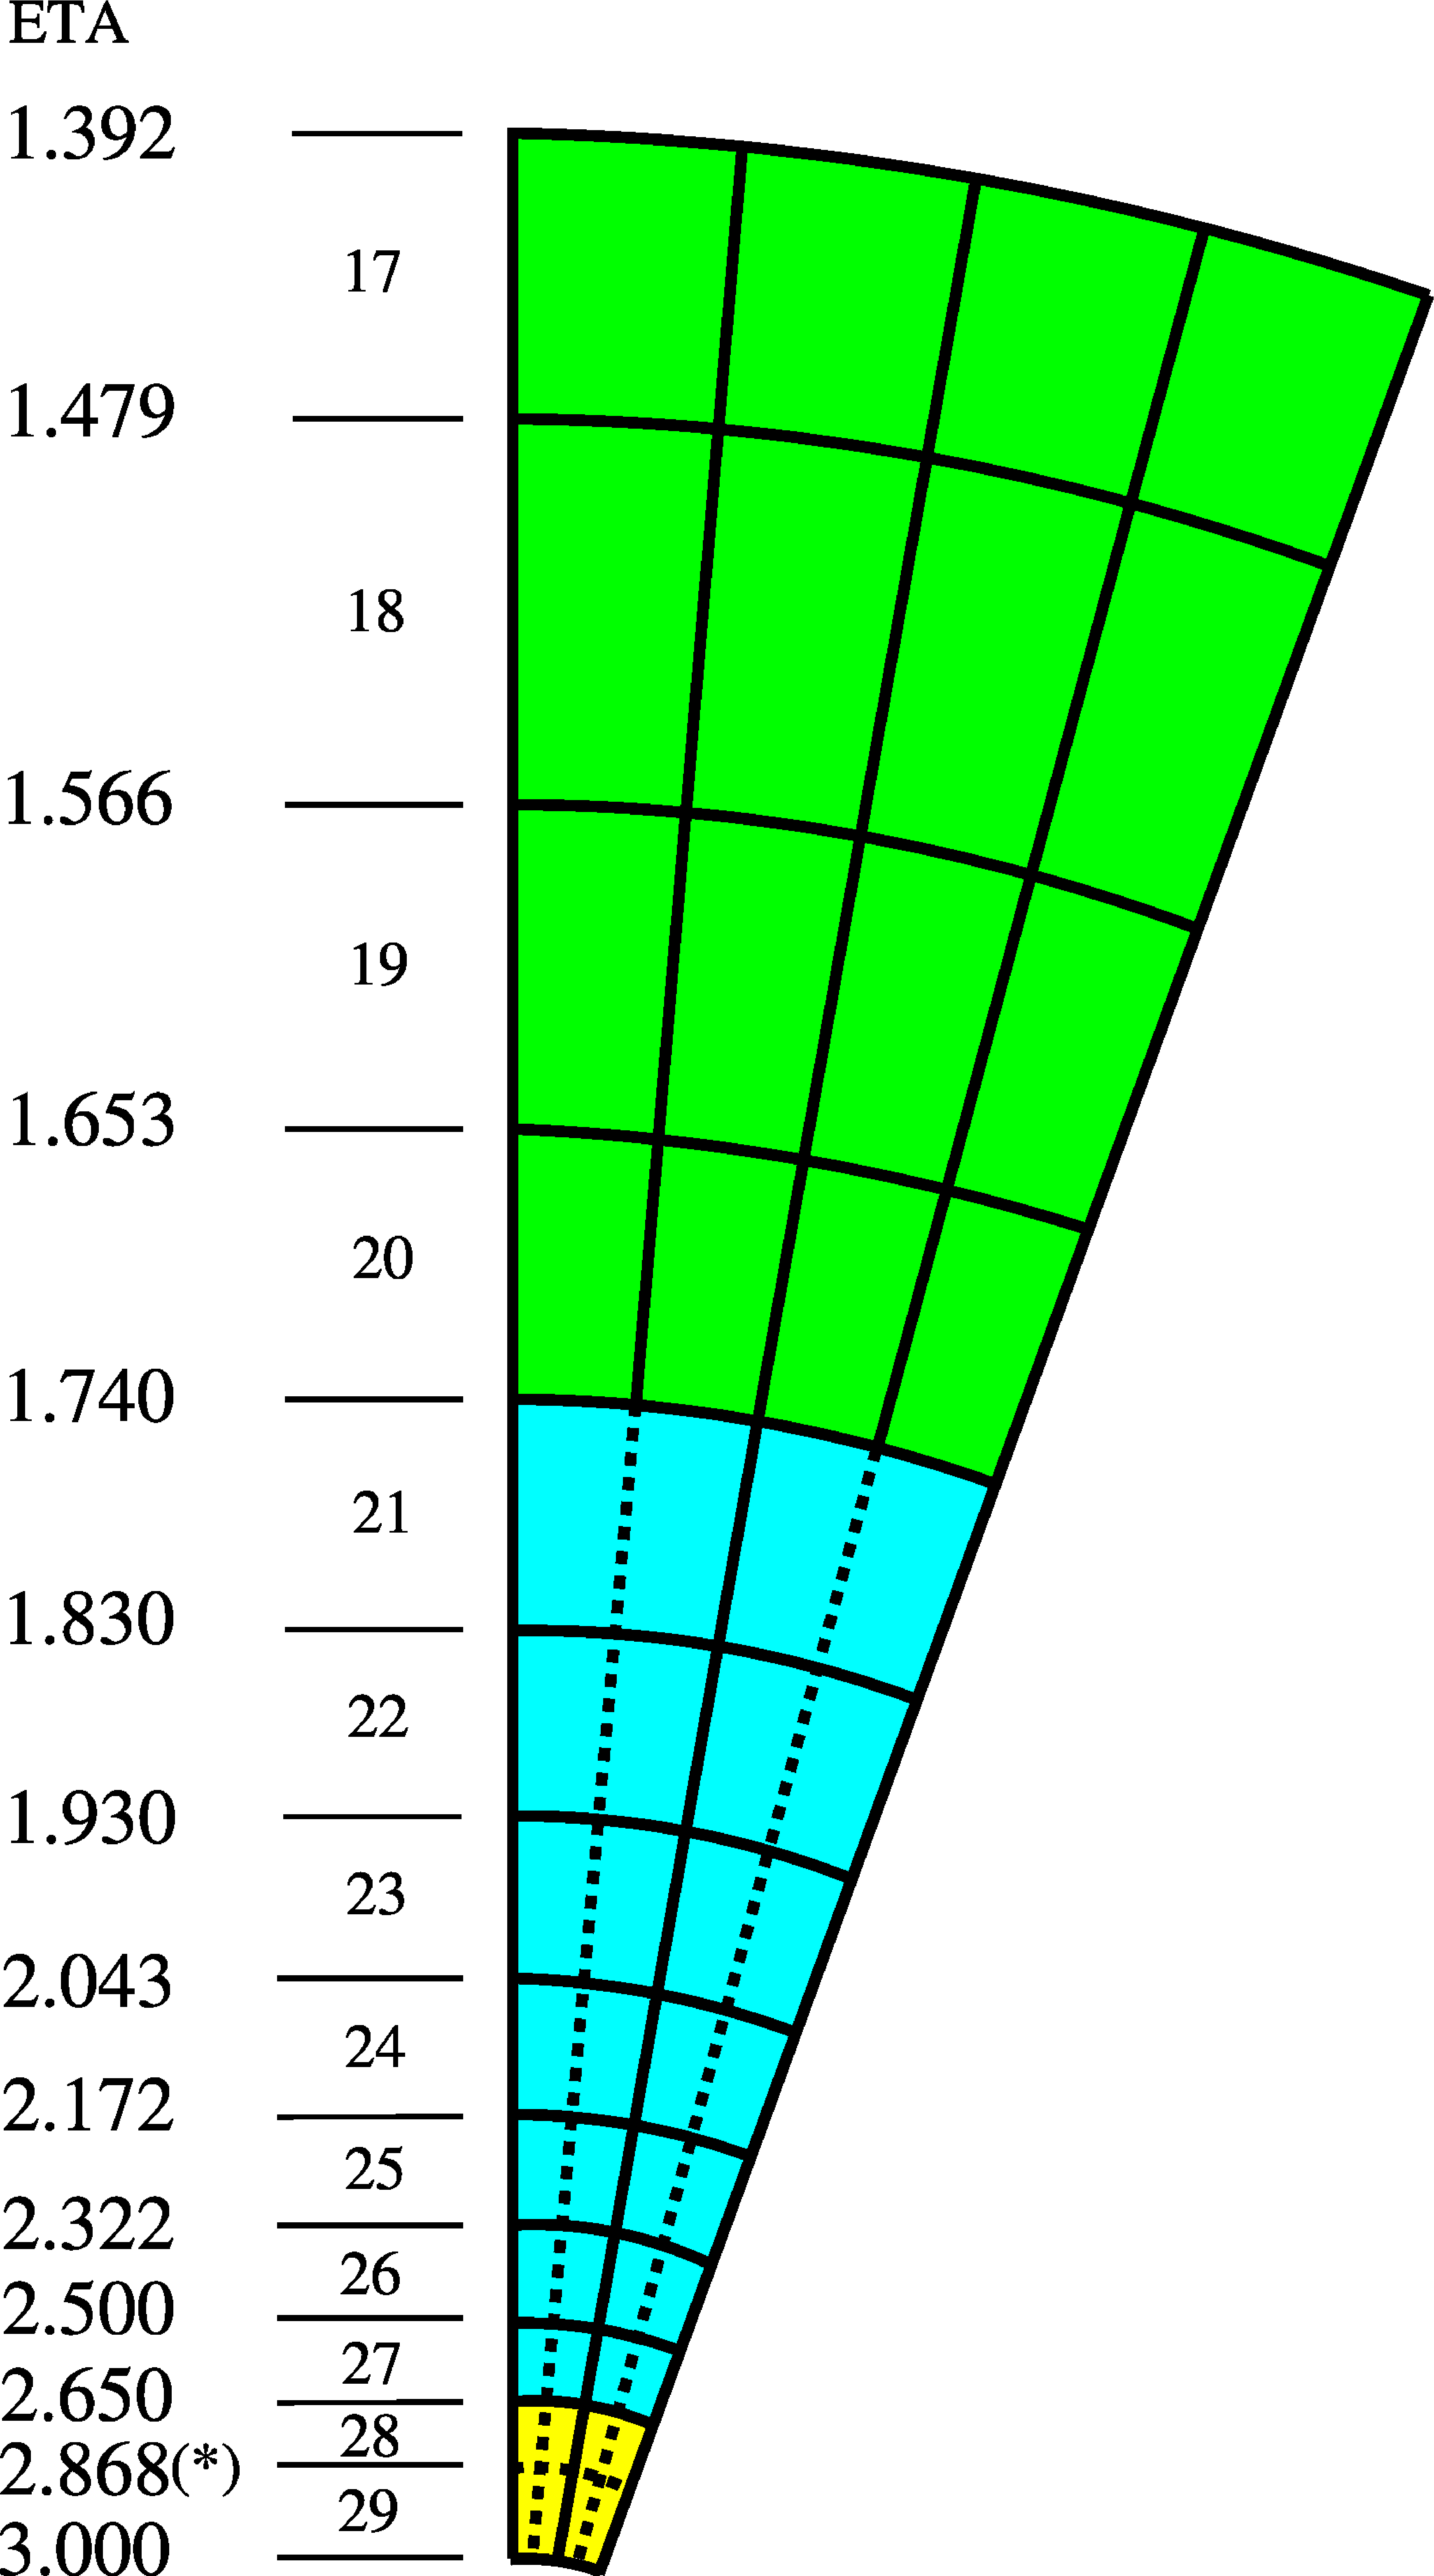
\includegraphics[width=0.35\textwidth]{figures/Figure_005-002-a.pdf} & 
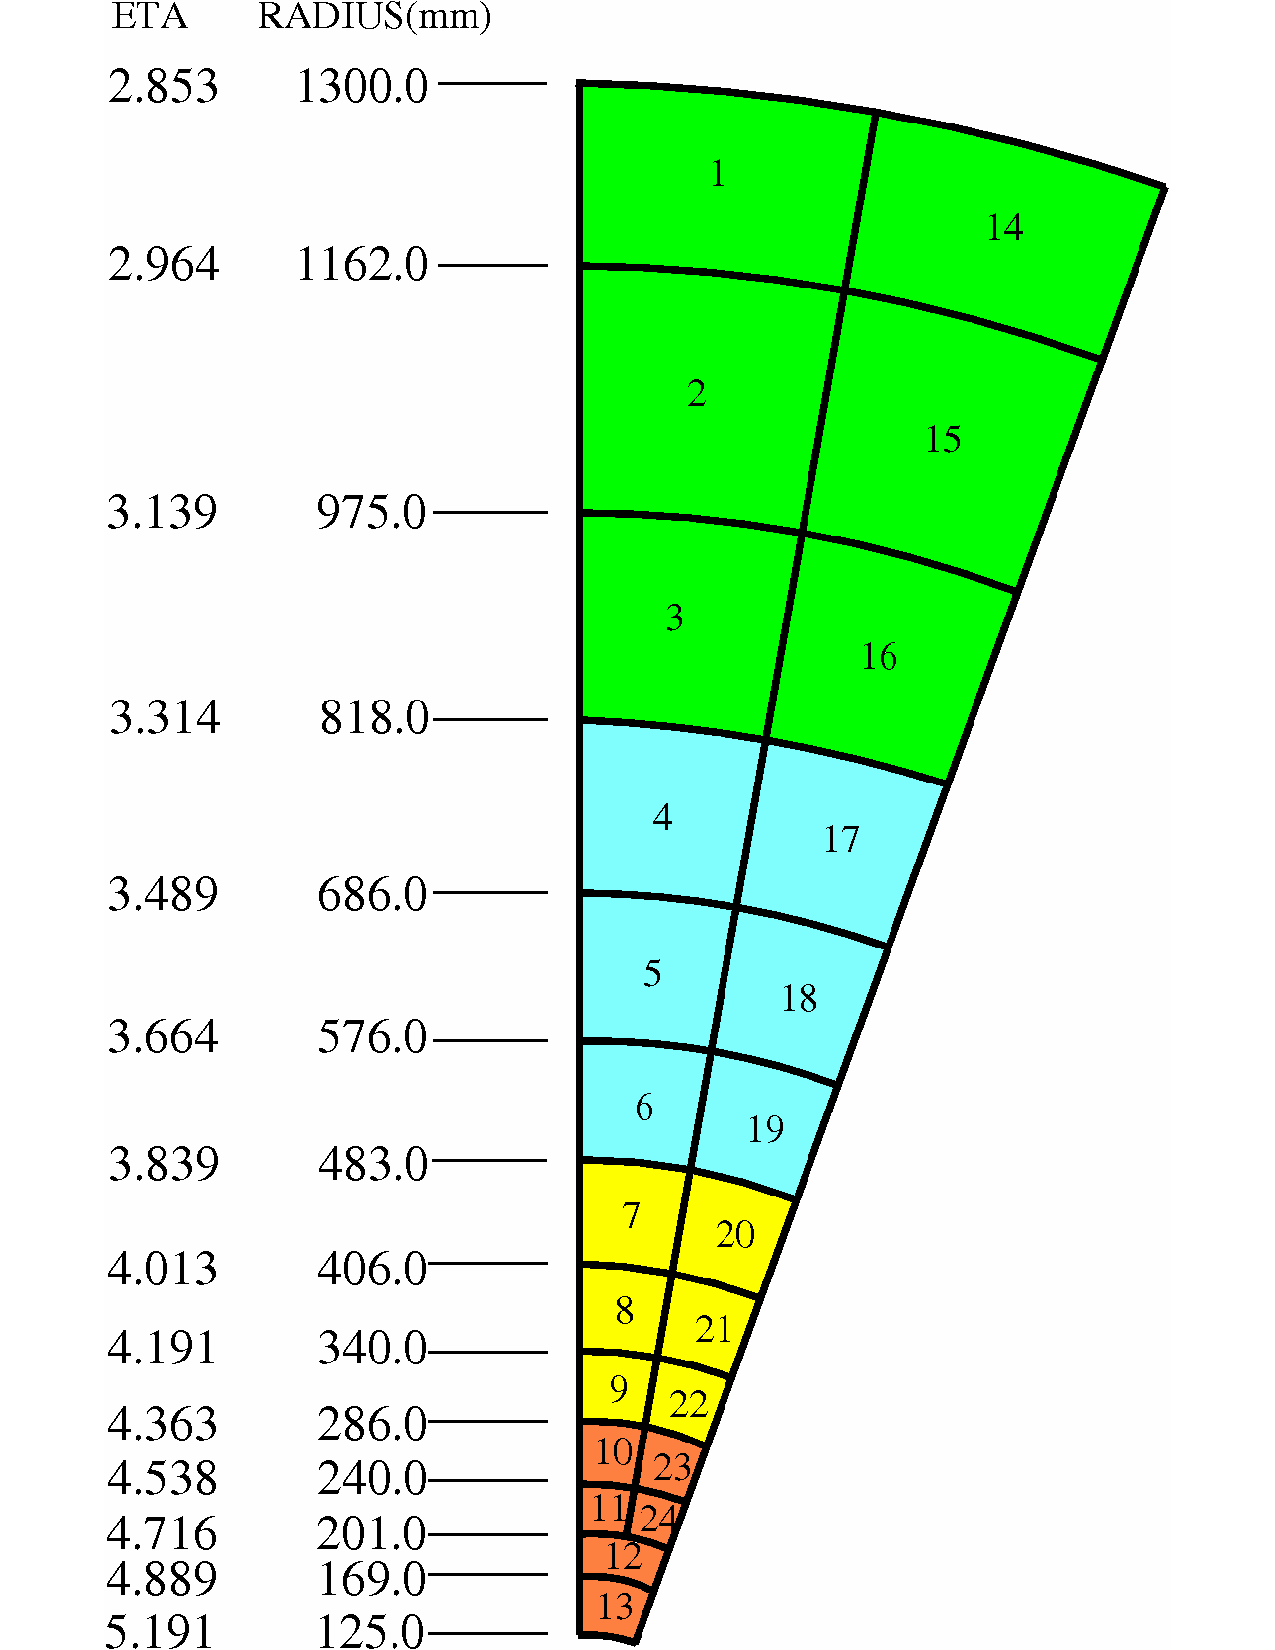
\includegraphics[width=0.47\textwidth]{figures/Figure_005-002-b.pdf} \\
%\hline
\end{tabular} 
\caption{Layout of a single wedge of HE(left) and HF(right)~\cite{cmstdr1}.}
\label{fig:hcal_HEHF} 
\end{figure} 

Fig.~\ref{fig:hcal_res} shows resolution of jet transverse energy 
in 3 different $|\eta|$ ranges(0-1.4, 1.4-3.0, 3.0-5.0). 
The resolution is measured using QCD dijet events generated by PYTHIA (version 6.226)
and matching to generator level jet reconstructed stable particles is done by $\Delta R < 0.2$. 
Jets are reconstructed using iterative cone algorithm with a cone size R = 0.5~\cite{}. 
%\textcolor{red}{why better resolution in the endcap?}
%
\begin{figure}[h] 
\vspace{1cm}
\centering 
\begin{tabular}{|c|} 
\hline
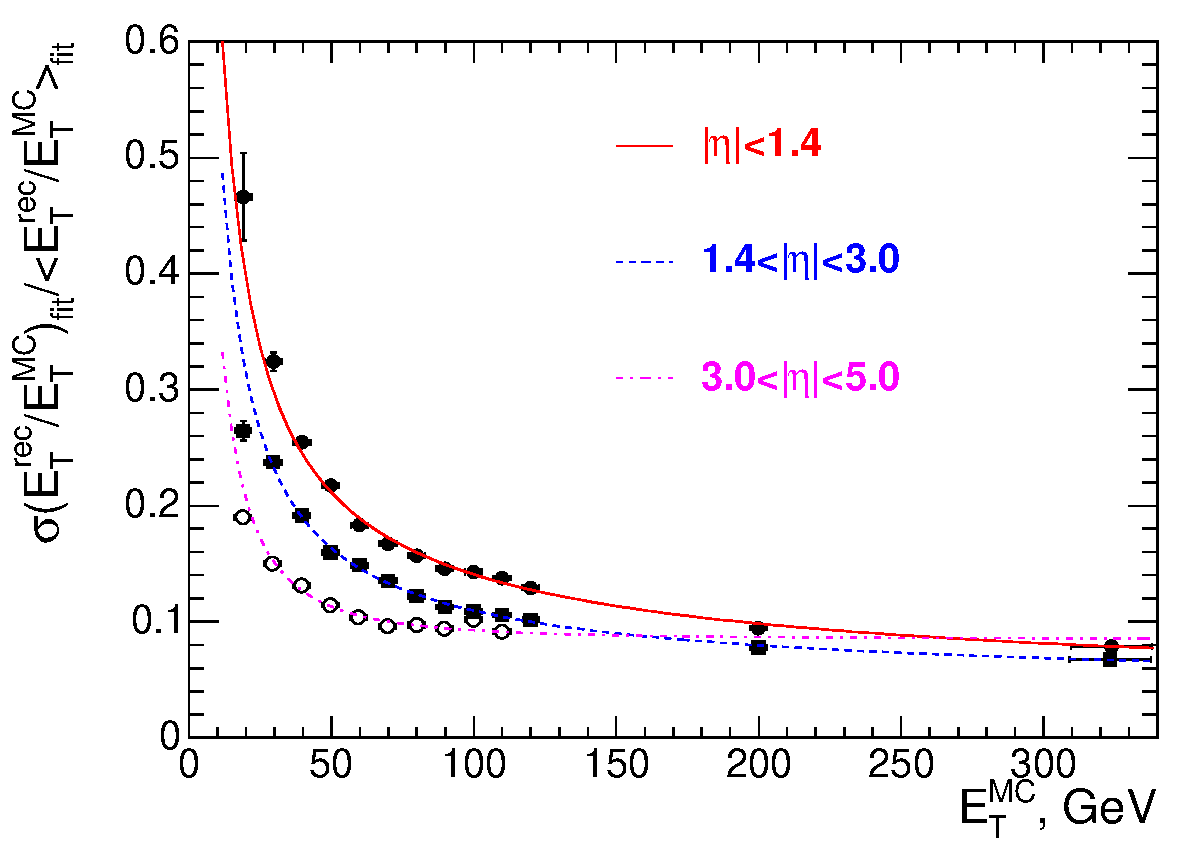
\includegraphics[width=0.6\textwidth]{figures/Figure_001-008.pdf}\\
\hline
\end{tabular} 
\caption{$E_T$ resolution of jets~\cite{cmstdr1}.}
\label{fig:hcal_res} 
\end{figure} 




%%%%%%%%
\subsection{Magnet} 

The momentum of a charge particle can be determined by measuring 
its curvature in magnetic field. Stronger magnetic field bends   
the trajectory more, thus allows better measurement of momentum.
CMS(as its names indicates) uses superconduncting solenoid 
which produces a uniform magnetic field  3.8(4.0 in design)~T 
in z direction. %\textcolor{red}{(or -z ?)}  
The solenoid has 2168 turns and the current to generate 3.8~T magnetic field  
is around 18~kA, giving a stored energy of 2.3~GJ. 
The size of the magnet system is 12.9~m in length and 5.9~m in diameter. 
The three layers of return yokes that guide the magnetic field back to the solenoid 
are installed outside of solenoid, interleaved with the muon system. 
The magnet system also provides mechanical support of the detector
because of its strength and tolerance to its own magnetic field. 
Fig.~\ref{fig:magnet} shows the photos of CMS magnet system : 
return yoke, outer vacuum tank and coil. 

%
\begin{figure}[h] 
\vspace{1cm}
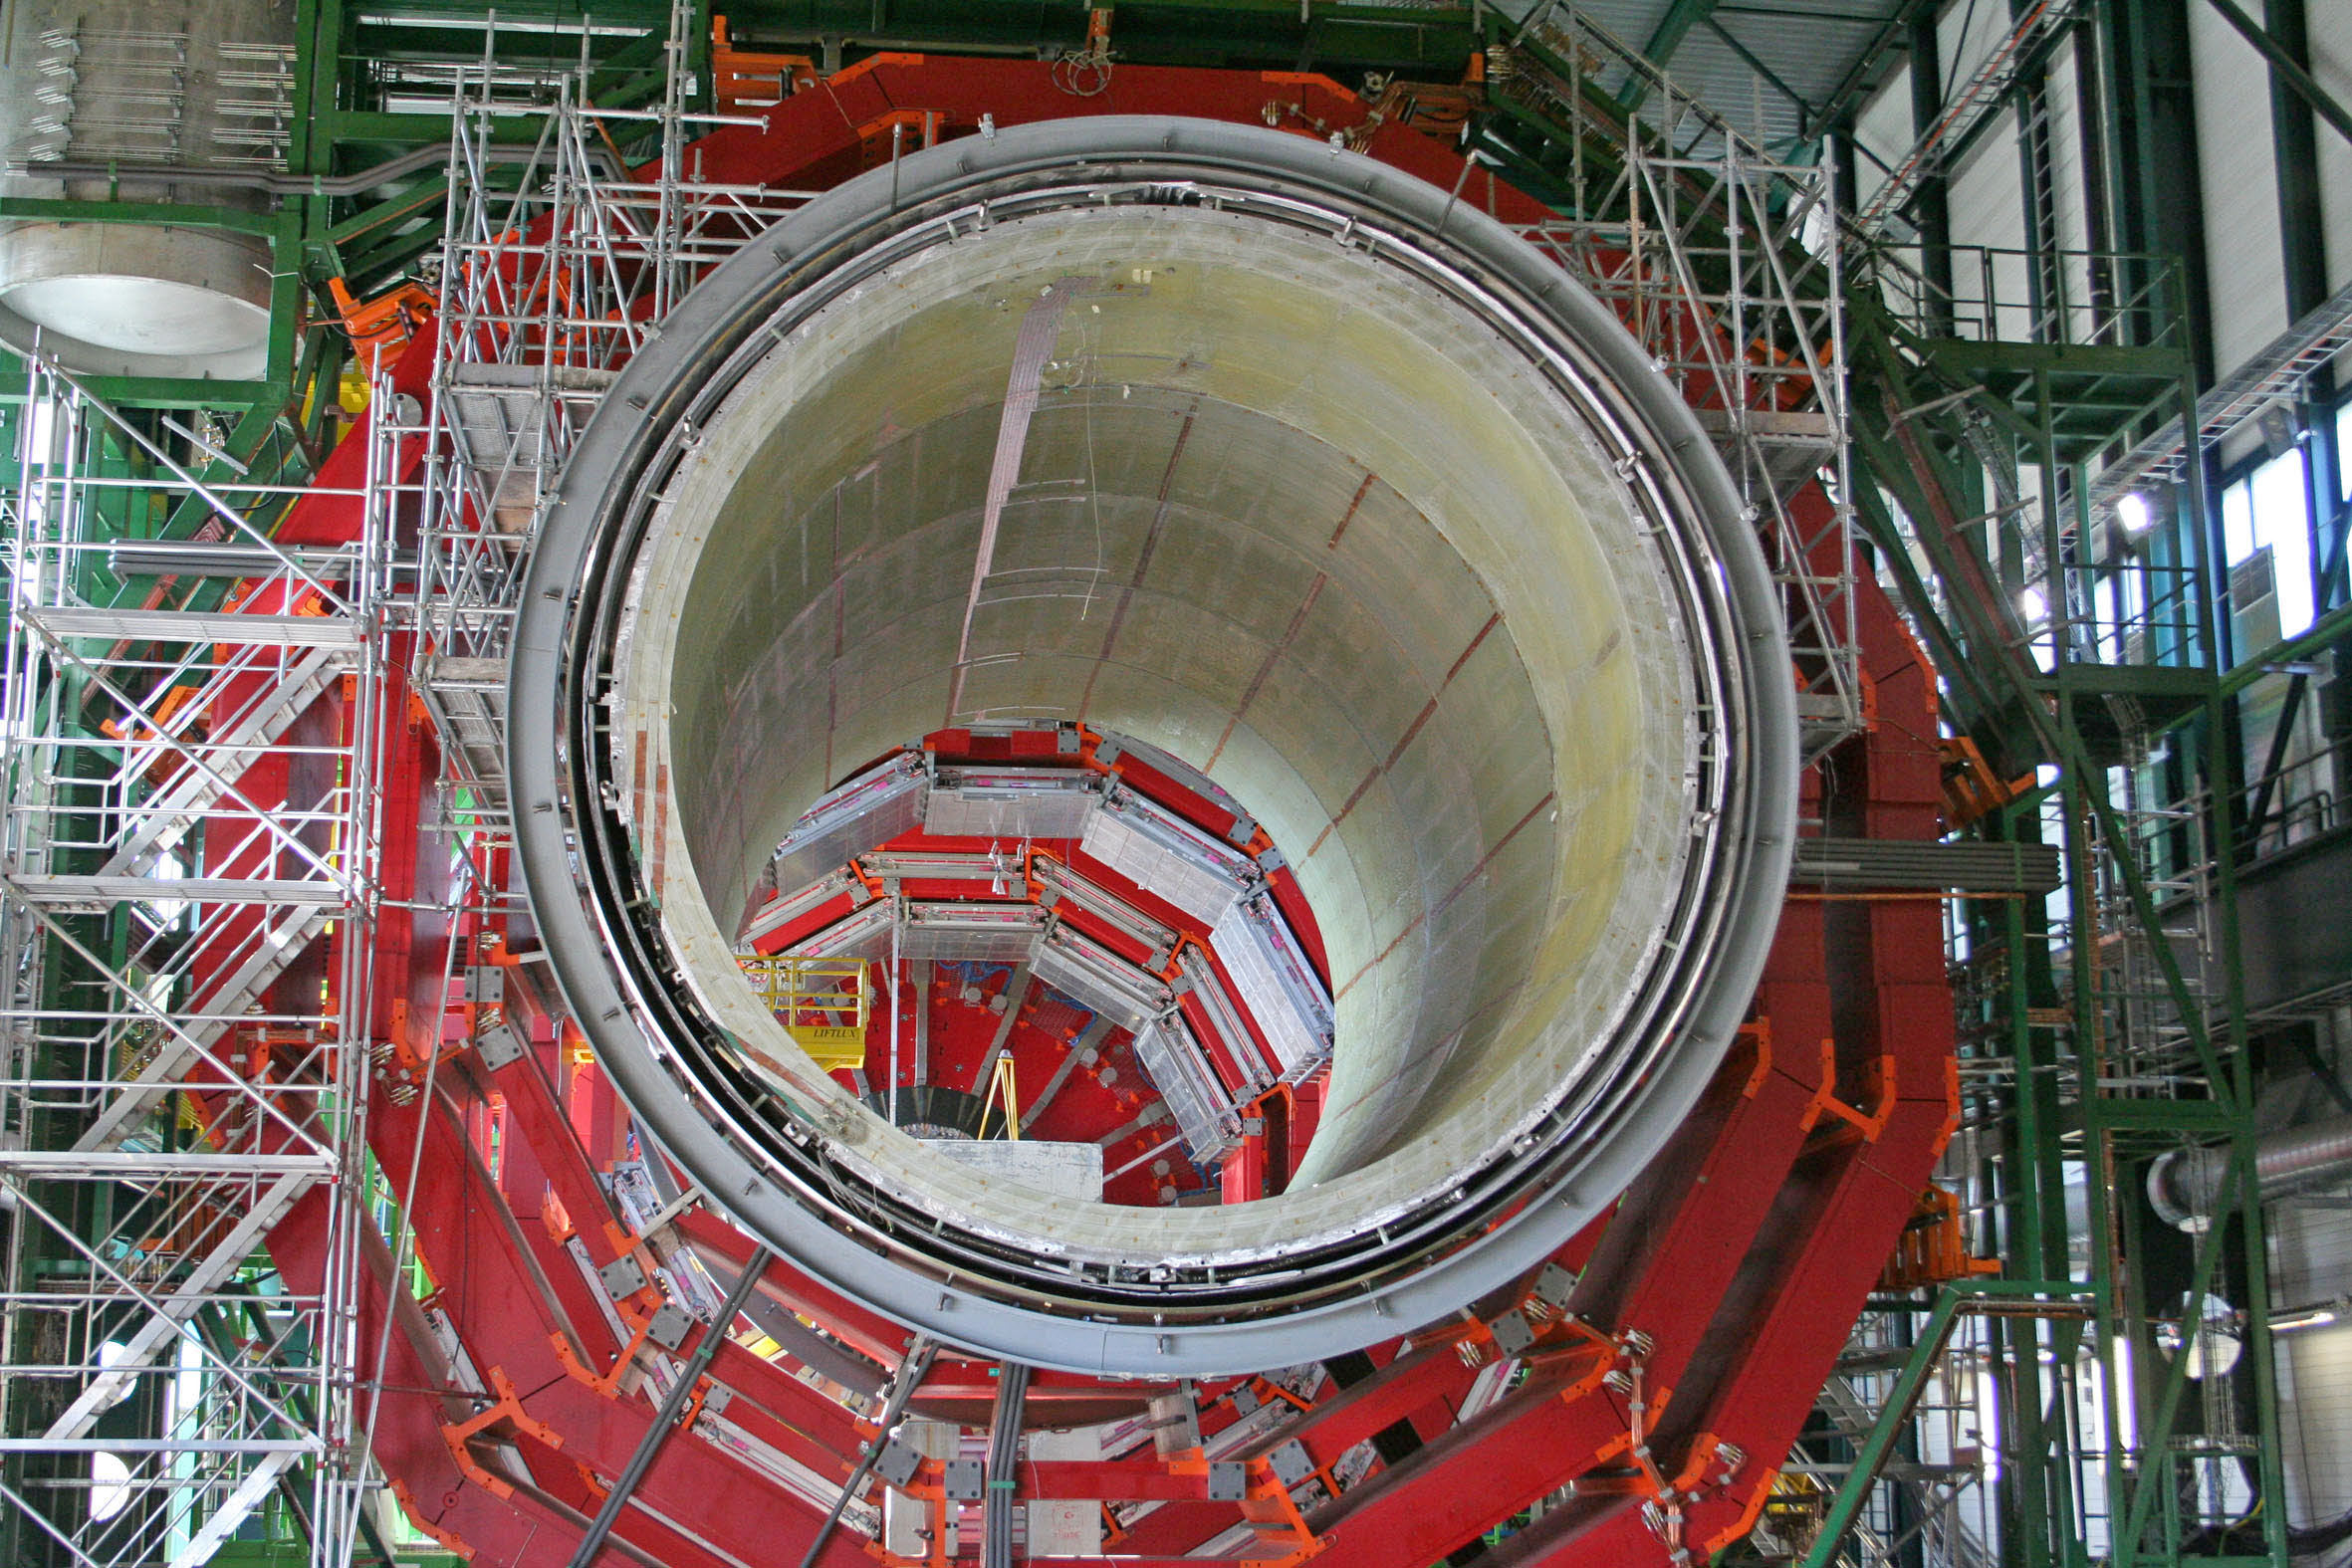
\includegraphics[width=0.99\textwidth]{figures/Figure_CP-1.jpg} \\
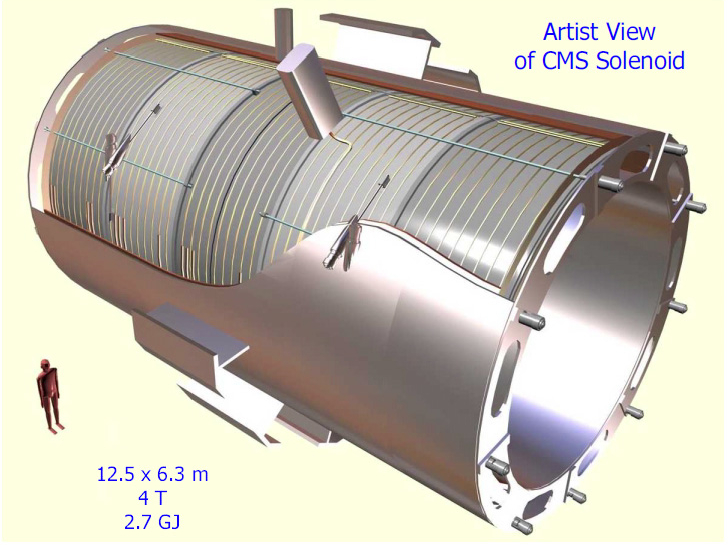
\includegraphics[width=0.49\textwidth]{figures/CMS-solenoid-magnet.jpg} 
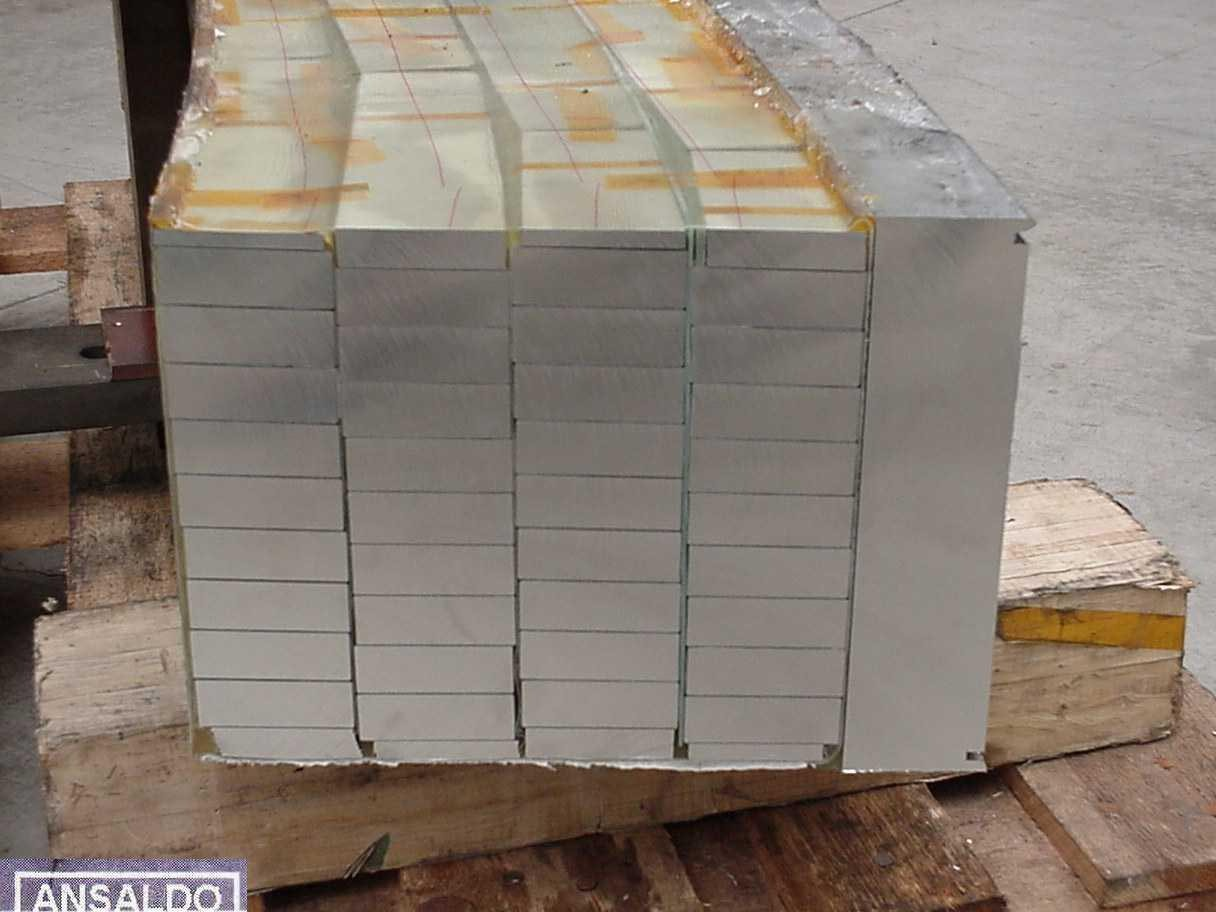
\includegraphics[width=0.49\textwidth]{figures/magnet-2000-049.jpg}
\caption{Magnet system of CMS~\cite{cmstdr1}. The top photo shows 
the the yoke(red), outer vacuum tank and the coil. The left bottom photon shows 
pictorial view of the magenet system and the right bottom photo shows 
the cross section of coils.}
\label{fig:magnet} 
\end{figure} 



%%%%%%%%
\subsection{Muon System} 

The Muon system of CMS is composed of three gaseous detectors, 
Drift Tube chambers(DT), Cathode Strip Chambers(CSC) and Resistive Plate Chambers(RPC) 
that cover $0<|\eta|<1.2$, $0.9<|\eta|<2.4$ and $0<|\eta|<1.6$, respectively.
Fig.~\ref{fig:muon_system} shows the layout of a quarter of muon system. 
Muon Barrel region(MB) has four layers of muon station interleaved with 
three layers of return yoke. Each layer has a cylinderical shape around 
the beam axis. There are 5 segments in z direction as the return yoke. 
Muon Endcap region(ME) also has four layers(disks) of muon stations
placed perpendicular to the beam axis.
The innermost disk(ME1) has 3 concentric rings and the other disks 
have 2 rings. 
%
\begin{figure}[h] 
\vspace{1cm}
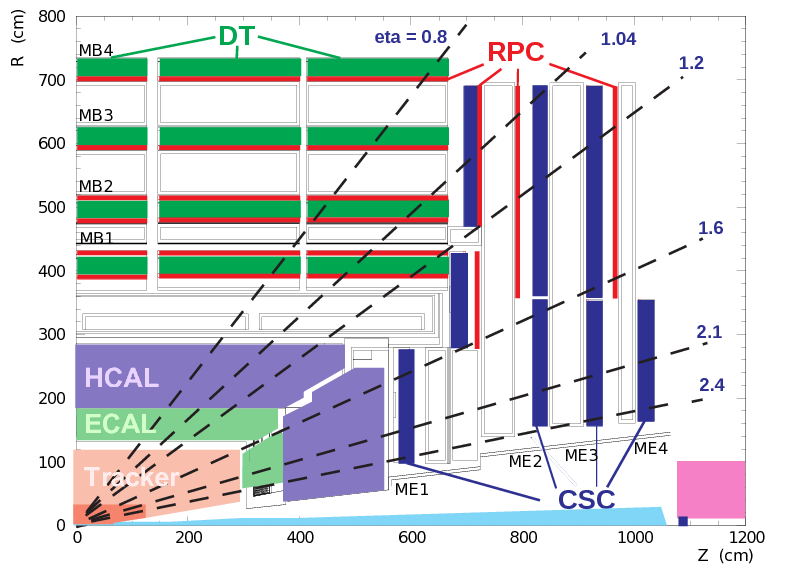
\includegraphics[width=0.99\textwidth]{figures/MuonSys-mod3.png}
\caption{Muon system~\cite{Kim:2012ix}.}
\label{fig:muon_system} 
\end{figure} 

DT chamber consists of 250 chambers constructed in 4 layers at r = 4.0, 4.9, 5.9 
and 7.0~m from the beam axis. Each chamber has 2 superlayers in $\phi$ and 
1 superlayer in z direction. Each superlayer has 4 layers of drift tubes. 
Each drift tube has the width of $\approx$ 4~\cm\ and the height of $\approx$ 1~\cm, 
and there is a streched wire(anode) in the middle of tube filled with a mixture of 
Ar and $\textrm{CO}_2$ gas. When a muon passes through a tube, it knocks 
electrons off the atoms of the gas, and they are drifted to the anode.
Each tube provides 2-dimensional measurement. One is given by the position of 
the central wire, and the other is given by the drift time of electrons divided by
drift speed. Fig.~\ref{fig:muon_dt} shows a schmetic of a 
movement of electrons in a tube and an illustration of a single tube with the
electric field lines. Each station provides $\phi$ precision better than 100~\um\ 
in positin and 1~mrad in direction. 
%
\begin{figure}[h] 
\centering
\vspace{1cm}
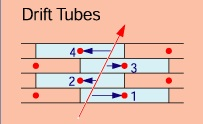
\includegraphics[height=0.3\textwidth]{figures/DT.jpg} 
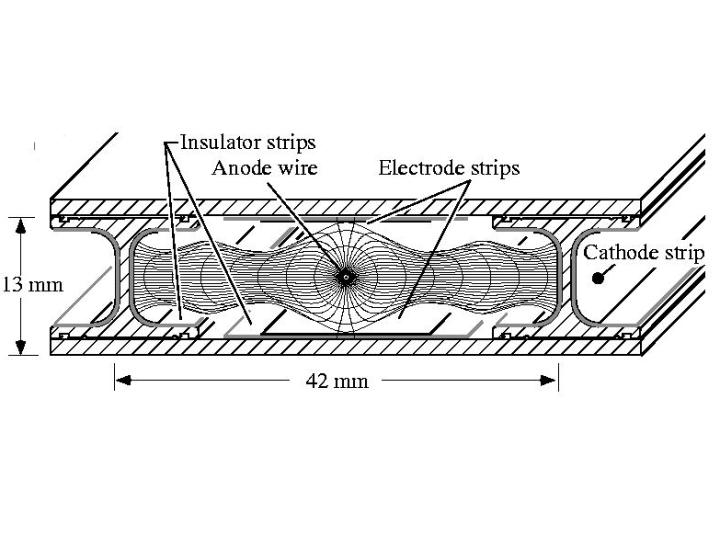
\includegraphics[height=0.3\textwidth]{figures/DT_onetube.jpg}
\caption{Schematic of a superlayer of DT(left) and a tube(right)~\cite{Maselli:1196170}.}
\label{fig:muon_dt} 
\end{figure} 

CSC is composed of 6 gas gaps filled with a mixture of Ar, $\textrm{CO}_2$ and $\textrm{CF}_4$,
and each gap has a plane of radial cathode and a plane of anode wires perpendicular 
tothe strips. The gap between the anode wires is about 3~mm and the width of a strip 
is 3-16~mm. Fig.~\ref{fig:muon_dt} shows a schematic of a CSC on the left 
and an illustration of what happens when a muon passes through a gas gap. 
When a muon tranverses in the gas, it knocks out electrons from the gas atoms. 
Then, an avalanche of electrons is created and moves to the wires.
The ionized positive atoms move toward the strips and make a charge pulse. 
Because the wires are the strips are laid perpendicular to each other, 
each gas gap provides 2-dimensional measurements. 
By weighting by charge distribution, a precise spatial measurements can be made. 
Each CSC provides spatial resolution of 200~\um\ using strips 
and $\phi$ resolution of order of 10~mrad.
Because of fast drift time, CSC is used in the Level-1 trigger. 
%
\begin{figure}[h] 
\centering
\vspace{1cm}
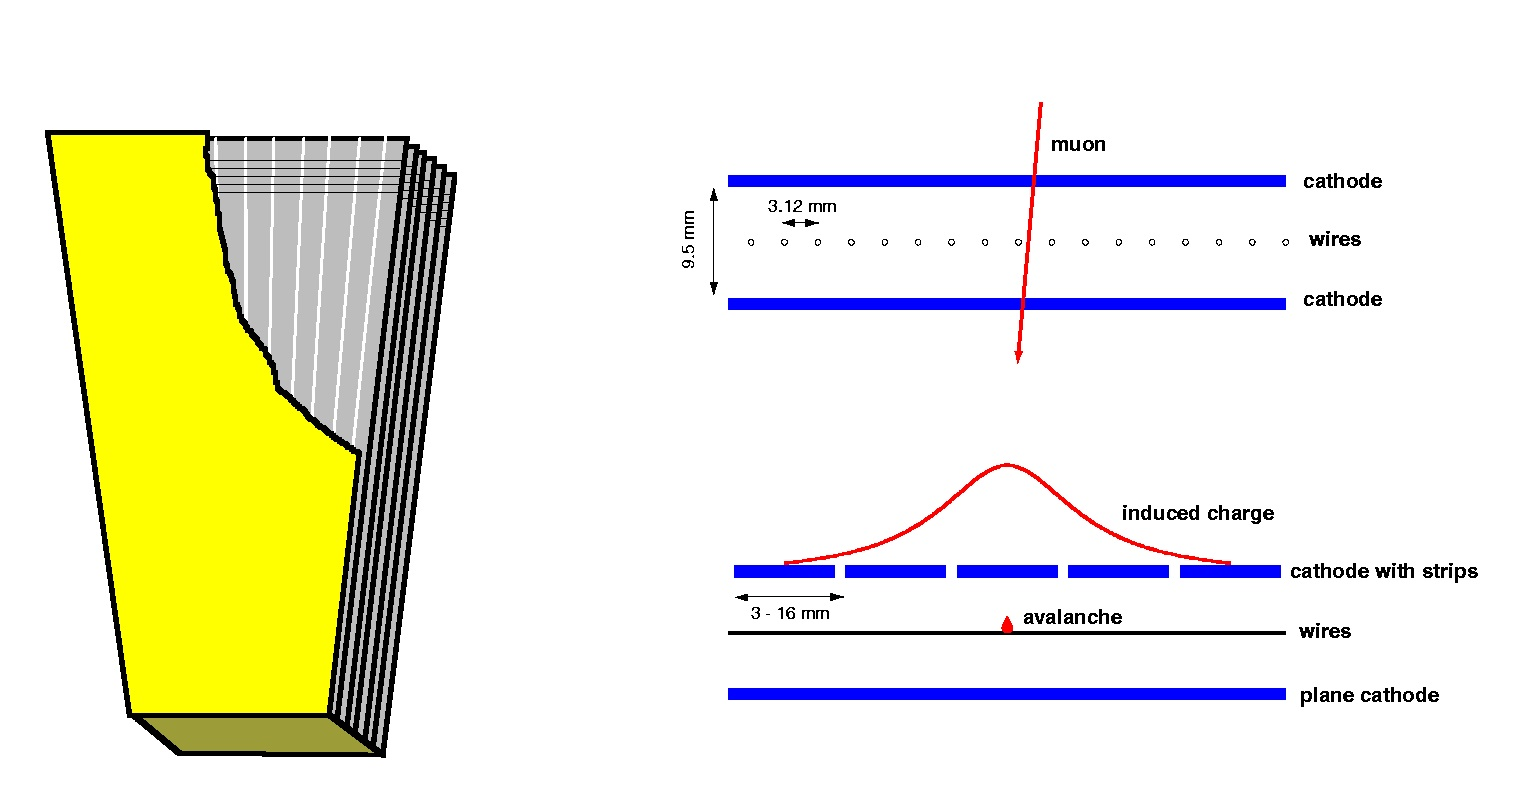
\includegraphics[width=0.99\textwidth]{figures/csc.jpg}
\caption{Schematic of CSC.}
\label{fig:muon_dt} 
\end{figure} 

RPC has one anode plate and one cathode plate organized in parallel
as shown in fig.~\ref{fig:muon_rpc}. 
The plates are separated by a gas chamber of thickness 2~mm 
filled with a mixture of $\textrm{C}_2\textrm{H}_2\textrm{F}_4$ 
and $\textrm{i-C}_2 \textrm{H}_{10}$.
When a muon passes through the chamber, an avalanche of electrons is formed, 
and the electrons are collected by external metallic strips. 
The pattern of the strip hits are then traslated to the momentum measurement
of the muon. Though the spatial resolution of RPC is not as good as DT or CSC,
its time resolution is very good(3~ns), thus it is able to identify 
correct bunch crossing without ambiguities. 
%
\begin{figure}[h] 
\centering
\vspace{1cm}
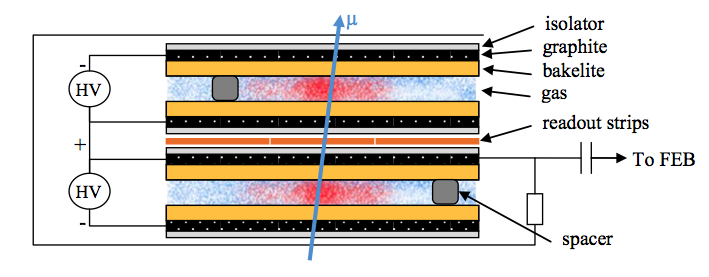
\includegraphics[width=0.99\textwidth]{figures/rpc.png}
\caption{Schematic of RPC~\cite{Lenzi:2013xpa}.}
\label{fig:muon_rpc} 
\end{figure} 


%%%%%%%%
\subsection{Trigger and Data Acquisition} 
% https://twiki.cern.ch/twiki/bin/view/CMSPublic/WorkBookHLTTutorial

The design bunch crossing rate of 40~Hz yiels $\sim 10^9$ events per second
at the design luminosity. However, only $\sim 100$ Hz of events can be recorded 
on the tape. So, the trigger system should attain about an order of $10^6$ 
reduction of events. CMS trigger and DAQ system is composed of 
detector electronics, Level-1(L1) triggers, readout networks and 
High-Level triggers(HLT). 

The time allocated to L1 trigger decision and data transit is 3.2~\um.
During this time, the data collected by detectors are kept in buffers 
until the decision is made. The decistion is made based on the presence 
of trigger primitives such as photons, electrons, muons and jets 
in the kinematic region of interests. It also employs global sums 
of $E_T$ and \met. Custum hardware processors are used for L1 decision.  
L1 reduces the crossing rate by an order of 1000 targeting 100~kHz.  

Once the L1 decision is made, after further processings, 
the data on the buffer is transferred to the front-end memories for access 
by the DAQ system. The data for an event is sent to a processor 
in a computing farm with $\mathcal{O}(10^3)$ processors. 
Each processor runs the same HLT software to reduce the L1 rate 100~kHz 
down to 100~Hz. The HLT software uses partial event reconstruction, 
and makes decision combining information from multiple virtual trigger 
levels, for example, L2 for calorimeter and muon and L3 for tracking. 
The use of HLT after L1 gives a maximal flexibility because 
it gives freedom in selection. 



%%%%%%%%
\subsection{CMS computing}  
% https://twiki.cern.ch/twiki/bin/view/CMSPublic/WorkBookComputingModel
% https://twiki.cern.ch/twiki/bin/view/CMSPublic/WorkBookCMSSWFramework

Even after the rate of data recording is reduced to 100~Hz by HLT, 
it is still a huge amount of data to store and process. CMS thus employed 
highly distributed computing model(grid system) with Tier-0 center at CERN supplemented 
by Tier-1 and Tier-2 computing centers all around the world. 

Tier-0 center repacks RAW data into primary datasets using trigger information
and send them to Tier-1 centers. It also does prompt reconstruction 
that produces RECO and Analysis Object Data(AOD),
and distribute them to Tier-1. Tier-0 is not accessible by analysers, but  
performs only scheduled activities. 
Tier-1 centers stores a subset of RAW data as backup, provides CPU power for 
re-reconstruction, skimming, calibration and AOD extraction, and 
stores and distributes the produced datasets to Tier-0 or Tier-2. 
Tier-2 centers participate in MC production organized by Tier-1 and 
send the produced MC samples to Tier-1 for distribution in the CMS collaboration. 
Other than this task, Tier-2 serves analysers by providing local computing 
resources as well as grid-based analysis support for the whole experiment.  
